% Local Variables:
%   compile-command: 
%     "xelatex -syntex=1 main.tex"
% End:
\documentclass[prodmode,acmtecs]{acmsmall}
% This is "sig-alternate.tex" V1.3 OCTOBER 2002
% This file should be compiled with V1.6 of "sig-alternate.cls" OCTOBER 2002
%
% This example file demonstrates the use of the 'sig-alternate.cls'
% V1.6 LaTeX2e document class file. It is for those submitting
% articles to ACM Conference Proceedings WHO DO NOT WISH TO
% STRICTLY ADHERE TO THE SIGS (PUBS-BOARD-ENDORSED) STYLE.
% The 'sig-alternate.cls' file will produce a similar-looking,
% albeit, 'tighter' paper resulting in, invariably, fewer pages.
%
% ----------------------------------------------------------------------------------------------------------------
%% latex main2.tex
%% dvipdfmx main
% Package to generate and customize Algorithm as per ACM style
\usepackage[ruled]{algorithm2e}
\renewcommand{\algorithmcfname}{ALGORITHM}
%%\usepackage{algorithm}

\usepackage{amsmath, amssymb}

\usepackage{algorithmic}
\usepackage{tikz}
\usetikzlibrary{external}
\usetikzlibrary{shapes,arrows}
\usetikzlibrary{matrix}
%  \Pdfpagewidth=8.5truein
%  \pdfpageheight=11truein

%\usepackage{graphics}

%%\usepackage[protrusion=true,expansion=true]{microtype}


\usepackage{caption}
\DeclareCaptionType{copyrightbox}
\usepackage{standalone}
\usepackage{enumerate}
\usepackage{turnstile}

\usepackage{booktabs}
%Use displaystyle everywhere
\everymath{\displaystyle}
%\newdef{definition}{Definition}

\SetAlFnt{\small}
\SetAlCapFnt{\small}
\SetAlCapNameFnt{\small}
\SetAlCapHSkip{0pt}
\IncMargin{-\parindent}

% Metadata Information
\acmVolume{9}
\acmNumber{4}
\acmArticle{39}
\acmYear{2010}
\acmMonth{3}

% Document starts
\begin{document}

% Page heads
\markboth{K. Katayama et al.}{Finding All Subgraph Isomorphisms Efficiently In a Large Database}
%
% Title portion
\title{Finding All Subgraph Isomorphisms Efficiently In a Large Database}
 
\author{Kaoru Katayama
\affil{Tokyo Metropolitan University}
Ernest Weke Maina
\affil{Tokyo Metropolitan University}}

\begin{abstract}


We study the problem of efficient enumeration of all subgraph isomorphisms of database graphs that exist in a query graph. We start by storing the graph database in a Directed Acyclic Graph (DAG) data structure. This allows  nodes represent unique subgraphs of the database graphs. Usidng this structure we formulate a fast algorithm for decomposing and searching for subgraphs in large database scalably.

%We study the problem of scalable enumeration of all subgraph isomorphisms to a query graph that exist in a graph database. We  propose several improvements and extensions to known algorithms to solve this problem that result in order of magnitude improvement in scalability. 
Graphs have become increasingly important structures for representing and understanding complex structures. Enumeration of subgraphs requires deciding whether a graph is a subgraph of another graph is called the subgraph isomorphism problem and is NP complete. In this study we are concerned with the efficient enumeration of all subgraphs of a query isomorphic to the graphs in a database. 
%In this study we are concerned with the enumeration of all subgraph isomorphisms of query subgraphs that are present in a graph database.

%We define the enumeration of isomorphic subgraphs to satisfy two conditions. First, a decision whether or not a graph isomorphic to a subgraph of a query graph exists in the graph database. 
%Second, for each graph in the database we find all instances of isomorphic subgraphs in the query. 
However mere detection of subgraph isomorphisms requires subgraph isomorphism tests that are known to be NP-complete. Additional Search for features multiple times in the query graph also results in redundant computation.
%However the retrieval of all subgraph isomorphisms is complicated and expensive because the subgraph isomorphism problem is NP-complete.

Recently, there have been several studies on efficiency of detection of subgraph isomorphisms of a query from a graph database but few have considered decomposition methodology to reduce the larger, difficult graph matching problem to smaller more managable sub-problems in a divide and conquer fashion. 

%%Messmer et al. studied an interesting method for retrieval of induced subgraph isomorphisms of a query graph. They proposed a so-called \textit{Network Method} that stores graphs  in a network structure  by recursively decomposing the individual graphs in a divide and conquer fashion, and the algorithms to facilitate retrieval using the structure.

% for the \textit{Network Method} and extend it to cover retrieval of non-induced subgraph isomorphisms of a query graph. 
We propose a new method of decomposition and subgraph processing to facilitate subgraph isomorphism queries. First, we recursively decompose at random  the query graph. Each decomposition is immediately followed by redistribution of resulting graph fragments so that only two subgraphs result. This subgraph decomposition without fragmentation process is efficient for both positive queries, where the database graphs is isomorphic to a subgraph of query and non-positive queries where no subgraph isomorphism exists. For positive queries, our method is efficient due to the compact representation of unique common subgraphs in the DAG  and recursive processing, both of which remove redundant computation. This is also the case for non-positive queries since computation is minimized by the recursive processing that allows early termination of computation. Repeated decomposition and redistribution for each node on DAG data structure amplifies these desirable properties. 

% \textit{Fast  Network Method}
%%recombining and reordering of the graph fragments to restrict decomposed graph count and maximize decomposed graph size. 

%We validate our proposed method experimentally. The result 
An extensive empirical study demonstrates the efficiency and scalability of the proposed methods. We achieve  an order of magnitude improvement in scalability over existing method for all subgraph isomorphism enumeration.
% for larger query graphs of up to 500 nodes and a database of 20,000 graphs. 
We also show a substantial improvement even when compared to state-of-the-art subgraph isomorphism detection-only algorithms. 

%Our method is particularly suited to larger query graphs or very larger graph databases.

%Graphs have become increasingly ubiquitous and very important structures for representing and understanding complex structures. In many cases the decomposition of Graphs and their representation has become central problem affecting the tractability of graph search algorithms. Traditional graph search 


Graphs have become increasingly important structures for representing and understanding complex structures.
We study the problem of scalably enumerating all subgraph isomorphisms of a query graph that exist in a graph database.

We start by constructing a graph database by decomposing database graphs and storing all the subgraphs at the nodes of a Directed Acyclic Graph (DAG).

Using the DAG data structure we apply three rules to reduce unnecessary computation of subgraph isomorphism. First, if all the nodes in the database graph do not exist in the query then that database graph is not a subgraph of the query graph. Secondly, if any subgraph of the database graph does not exist in the query graph, the database graph is not a subgraph of the query graph. Thirdly, if a common subgraph of some database graphs does not exist in the query graph, none of the database graphs is a subgraph of the query graph.

The rules are implemented as a traversal of the DAG data structure. 

We present experimental results where we compare our proposed algorithms with two well known algorithms, all isomorphism enumeration by Messmer et. al as well as a state of the art isomorphism detection only algorithm, VF2. Results show an order of magnitude improvement in scalability over Messmer et.al. as well as substantial improvement over the VF2 algorithm despite the increased workload of enumerating all subgraph isomorphisms. Our method is particularly suited to larger query graphs or very larger graph databases




\end{abstract}

\category{C.2.2}{Computer-Communication Networks}{Network Protocols}


\terms{Experientation, Algorithms, Performance}

\keywords{Graph Database, Graph Decomposition, Subgraph Isomorphism}

\acmformat{Katayama, K., and Maina, E.W.,2011. Finding All Subgraph Isomorphisms Efficiently In a Large Database.}

\begin{bottomstuff}
This work is supported by the National Science Foundation, under
grant CNS-0435060, grant CCR-0325197 and grant EN-CS-0329609.

Author's addresses: K. Katayama {and} E.W. Maina, Graduate School of System Design,
Tokyo Metropolitan University.
\end{bottomstuff}

%\date{08 April 2011}
\maketitle


%\terms{Algorithms, Experimentation, Performance}

 

\section{Introduction}
%%Efficient algorithms for supergrap query processing on graph databases Shou Zhang, Xiaofeng Gao, Weili Wu, Jianzhong Li, Hong Gao, 2009.
The power and importance of graph structures is clearly evident in the numerous and varied use of graphs in such applications as: modeling of proteins
\cite{chi_muntz_nijssen2005}, molecular structures of compounds in chemistry\cite{willet_barnard_john1998}\cite{agrafiotis2007}, organization of entities 
in images\cite{petrakis_faloutsos1997} \cite{burge_kropatsch1999}, representation of components in computer aided design (CAD) drawings \cite{cordella2000}, 
topology of sensor networks\cite{li_wan_wang2003},and social and information networks\cite{cai_he_yan2005}. As a result a tremendous amount of structured 
data is being accumulated in large databases. An essential problem in managing the large amount of graphs and graph queries is the efficiency of query 
processing. In this article we address the problem of scalable enumeration of all subgraph isomorphisms existing in a database of graphs.

A subproblem of the subgraph isomorphism enumeration problem is the issue of deciding whether a graph contains another graph, which is called the 
\textit{subgraph isomorphism problem}. A subgraph isomorphism exist between two 
graphs if there exists one-to-one mapping between the smaller graph and a subgraph of the larger graph such that edge the adjacencies are preserved. 
Testing for subgraph isomorphism for an $n$-node graph in an $m$-node larger graph is a combinatorial matching exercise with $m^n$ possibilities, hence it is 
expensive. Therefore for a given query, evaluating a database for subgraph  isomorphism by individually testing each graph  in the database is 
inefficient.  In fact, the subgraph isomorphism problem is known to be NP-complete \cite{cook1971_np}. Enumeration of all subgraph isomorphisms clearly requires 
solving the subgraph isomorphism problem multiple times, one for each instance of isomorphism at the very least. In  many cases, the graph database is also very 
large which makes it necessary to build a framework to facilitate efficient query processing.

There are two basic approaches that past research has taken regarding the problem of finding graph and subgraph isomorphisms. The first approach is based on 
group theoretic concepts and aims to classify the adjacency matrices of graphs into permutation groups. With this, it is possible to prove that there exists 
a moderately exponential bound for the general graph isomorphism problem \cite{babai1981}. Also, by imposing certain restrictions on graphs it is possible to 
derive algorithms that have polynomial bound on complexity. For example  Luks and Hoffman\cite{hoffmann1982} describe a polynomially bound method for the 
isomorphism detection of graphs with bounded valence. These methods, though theoretically interesting, in practice they have a large constant overhead and 
are therefore impractical. They also apply only to graph isomorphism detection, but not the detection and enumeration of subgraph isomorphism which is 
required for a wide range of applications.

The second approach to graph and subgraph isomorphism is the use of heuristics for graph matching. This approach is  more practically oriented and aims 
directly at developing practical procedures. Most of the algorithms are based on search tree with backtracking. One of the first publications in this 
field was Corniel and Gotlieb \cite{corneil1970}. A major improvement of the bactracking method was then presented by Ullmann, who introduced  a refinement 
method which reduces the search space of the backtracking procedure remarkably \cite{ullmann1976}.

The methods for finding subgraph isomorphism mentioned so far work only with two graphs at a time. However in many applications there is more than 
one model that must be matched with the input graph. Consequently it is necessary to apply the subgraph isomorphism algorithm to each input pair 
resulting in a computation time that is linearly dependent on the size of the database. This dependency becomes prohibitive when the number of graphs 
in the database is large.  

A newer method for searching for all subgraphs is to first construct a database of the graphs to search for and the process the query over the database. In this
an efficient method to determing all possible matches over a large database is useful. Such a method is the Rete Matching Algorithm proposed by Forgy et. al. 
 in the filed of production rules. These algorithm is efficient because it compiles all the patterns into a tree structure. avoids iterating over the dataset by  

We can classify a third, more recent and Approach. This is represented by the network based approach to graph detection proposed by Messmer and Bunke
\cite{messmer_bunke2000} . In the new approach the tree is replaced by a network whose nodes contain subgraphs of the model graphs and traversing the 
network is equivalent to constructing a graph from the subgraphs. In this method, a powerful tool for obtaining efficient solutions to graph isomorphism 
detection, enumeration  and  problems is divide and conquer, which is expressed in the form of random graph decomposition. Decomposition techniques are 
an instantiation of the divide and conquer paradigm to overcome redundant work for independent partial problems. The main features of the Network based 
approach are as follows:

\begin{enumerate}
\item Offline decomposition of the model graphs into smaller graphs using  random decomposition
\item Decomposed subgraphs of model graph are saved in a network structure as the database. The process is repeated for all the model graphs in the database.
\item Subgraphs that appear in the same or multiple model graphs multiple times are represented in the network structure only once.
\item During graph matching the subgraphs are matched only once to the input graphs, the algorithm is only sublinearly dependent on the number of model graphs.
\end{enumerate}

For the above algorithms, given a database $D$ comprising of a set of graphs $g=g_1 ,g_2 ,\ldots g_n$ and query $Q$ consisting of a set of graphs 
$q=q_1 ,q_2 ,\ldots q_n$, there are, in general, two kinds of graph search problems that we can define. By far the traditional and the most popular 
one is the subgraph query. Given a graph database $D$ and a subgraph query $Q$ with  a query graph $q$, the answer to $Q$ is the set of $\{g \| g\in D$ 
and $q$ is a subgraph of $g\} $. The second search problem is a graph containment search where Given a graph database $D$ and a subgraph query $Q$ with  
a query graph $q$, the answer to $Q$ is the set of $\{g\ | g\in D$ and $q$ is a supergraph of $g\}$. Graph containment search with exclusion logic has 
recently become a  active area of research \cite{chen2007_cindex} \cite{zhang_gao_wu2011}.  
 

\begin{figure}
\centering
%& -shell-escape -enable-write18
\documentclass{standalone}
\usepackage{tikz}
\usetikzlibrary{external}
%\tikzexternalize
\usetikzlibrary{shapes,arrows}
\usepackage{caption}
\usetikzlibrary{matrix}
%\newcommand{mynodename}[#1]{\mathrm{#1}}\label{•} 
%\newcommand{mylabelleft}[#2]{label={[font=\fontsize{#1}{#1}\selectfont]above left:mynodename{#2}}}

\begin{document}
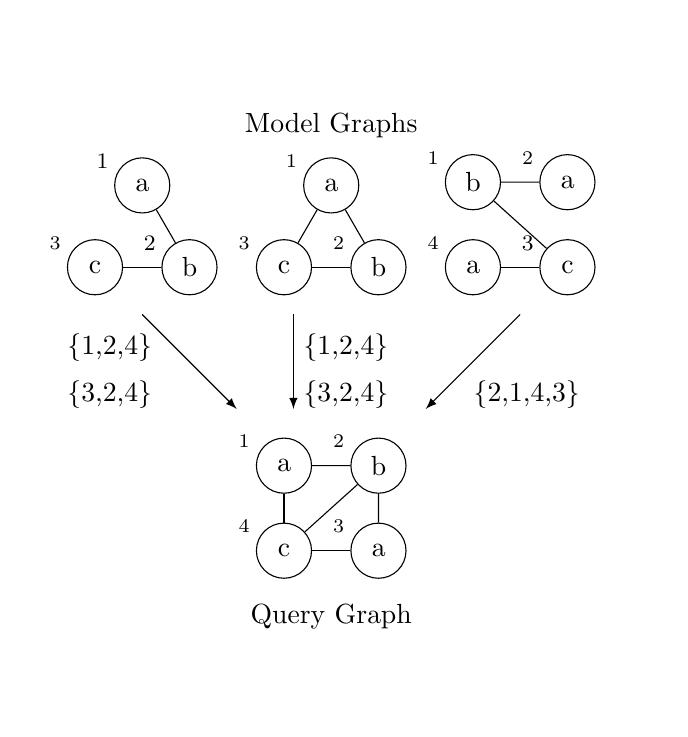
\begin{tikzpicture}[scale=1.2]
%[every node/.style={draw,circle}]
\tikzstyle{every node}=[draw,shape=circle,minimum size=0.7cm];
\tikzstyle{line} = [draw,-latex]
\colorlet{invisible}{white}
\colorlet{visible}{black}
%\tikzstyle{mylabelsfont=[font=\fontsize{7}{7}\selectfont,yshift=-.2cm];
%\tikzstyle{every label}=[text height=10pt];
\begin{scope}[shift={(0,-0.5)}] 
	\begin{scope}[yshift=0cm]% top row as a group
%	\draw[help lines] (-1,-6) grid (10,6);
	  \node (a) at (60:1cm) [label={[font=\fontsize{8}{8}\selectfont,yshift=-.2cm]above left:$1$}] {a};
	  \node (b) at (0:1cm)  [label={[font=\fontsize{8}{8}\selectfont,yshift=-.2cm]above left:$2$}] {b};
	  \node (c) at (0:0cm)  [label={[font=\fontsize{7}{7}\selectfont,yshift=-.2cm]above left:$3$}] {c};
	
	  \foreach \from/\to in {c/b,b/a}
	    \draw (\from) -- (\to);
	\end{scope}
	\begin{scope}[xshift=2cm]%top row middle
	  \node (a) at (60:1cm) [label={[font=\fontsize{7}{7}\selectfont,yshift=-.2cm]above left:$1$}] {a};
	  \node (b) at (0:1cm)  [label={[font=\fontsize{7}{7}\selectfont,yshift=-.2cm]above left:$2$}] {b};
	  \node (c) at (0:0cm)  [label={[font=\fontsize{7}{7}\selectfont,yshift=-.2cm]above left:$3$}] {c};
	
	  \node [draw=none] (query_label) at (0.5,1.5) {Model Graphs};% Model label
	  \foreach \from/\to in {c/b,b/a,c/a}
	    \draw (\from) -- (\to);
	\end{scope}
	\begin{scope}[xshift=4cm]%top row right
	  \node (a_1) at (0,0) [label={[font=\fontsize{7}{7}\selectfont,yshift=-.2cm]above left:$4$}] {a};
	  \node (b) at (0,.9)  [label={[font=\fontsize{7}{7}\selectfont,yshift=-.2cm]above left:$1$}] {b};
	  \node (c) at (1,0)   [label={[font=\fontsize{8}{8}\selectfont,yshift=-.2cm]above left:$3$}] {c};
	  \node (a_2) at (1,.9) [label={[font=\fontsize{7}{7}\selectfont,yshift=-.2cm]above left:$2$}] {a};
	
	  \foreach \from/\to in {a_1/c,c/b,b/a_2}
	    \draw (\from) -- (\to);
	\end{scope}
\end{scope}
\begin{scope}[shift={(0,0)}] % The arrow and bracket as a group
	\begin{scope}[shift={(0,-0.5)}]%just the arrows
		\path[line] (0.5,-0.5) -- (1.5,-1.5);
		\path[line] (2.1,-0.5) -- (2.1,-1.5);
		\path[line] (4.5,-0.5) -- (3.5,-1.5);
	\end{scope}
	\begin{scope}[shift={(0.5,-1.6)}]%annotations at left arrow
		\matrix (m)[matrix of nodes, column  sep=-1mm,color=visible,row  sep=-1mm, anchor=center,draw=none, nodes={rectangle,color=invisible,draw=none,text width = 2cm} ]{
\node [color=visible] {\{1,2,4\}};&\\
\node[color=visible]{\{3,2,4\}};& \\
};
	\end{scope}
	\begin{scope}[shift={(3.0,-1.6)}]%%annotations at middle arrow
	\matrix (m)[matrix of nodes, column  sep=-1mm,color=visible,row  sep=-1mm, anchor=center,draw=none,nodes={rectangle,color=invisible,draw=none,text width = 2cm} ]{
\node [color=visible] {\{1,2,4\}};&\\
\node[color=visible]{\{3,2,4\}};& \\
	};
	\end{scope}
	\begin{scope}[shift={(4.8,-1.6)}]%%annotations at right arrow
	\matrix (m)[matrix of nodes, column  sep=-1mm,color=visible,row  sep=-1mm, anchor=center,draw=none,nodes={rectangle,color=invisible,draw=none,text width = 2cm} ]{
\node [color=visible] {};&\\
\node[color=visible]{\{2,1,4,3\}};& \\
	};
	\end{scope}
\end{scope}

\begin{scope}[shift={(2,-3.5)}]%bottom row graph
  \node (a_3) at (1,0) [label={[font=\fontsize{7}{7}\selectfont,yshift=-.2cm]above left:$3$}] {a};
  \node (b) at (1,.9)  [label={[font=\fontsize{7}{7}\selectfont,yshift=-.2cm]above left:$2$}] {b};
  \node (c) at (0,0)   [label={[font=\fontsize{7}{7}\selectfont,yshift=-.2cm]above left:$4$}] {c};
  \node (a_4) at (0,.9) [label={[font=\fontsize{7}{7}\selectfont,yshift=-.2cm]above left:$1$}] {a};
  
  \node [draw=none] (query_label) at (.5,-.7) {Query Graph};% query graph label
  \foreach \from/\to in {a_3/c,a_3/b,c/b,c/a_4,b/a_4}
    \draw (\from) -- (\to);
    
\end{scope}
\end{tikzpicture}
\end{document}
\caption{Subgraph isomorphism query}
\label{fig:fig11}
\end{figure}


In this paper, we extend the method proposed by Messer et al.\cite{messmer_bunke2000}, so-called \textit{Network Method,(NA)}, to support \textit{subgraph isomorphism} queries.
Fig.\ref{fig:fig11} shows an example of a subgraph isomorphism query. We also reformulate a  \textit{Fast Network Method } to increase the scalability of this method.
Our main contributions are as follows.

\begin{enumerate}
\item The \textit{Network Method} originally only supports induced subgraph isomorphism query. We extend it  cover \textit{subgraph isomorphism} queries.
\item  In the \textit{Network Method}, much of graph decomposition is performed on graphs at random potentially creating many graph fragments. We add a new recombining 
process after each decomposition which is active when more than a pair of  subgraphs result from the decomposition.  Recombining results in exactly  two larger 
graphs for each decomposition step, where possible.  As a consequence, we are able to drastically reduce the potential rapid increase in matchings. 
\item We formulate and implement  a  \textit{Fast Network Method} on the offline preparation of the database. The new algorithm performs recombination 
on  each recursive decomposition in the  preprocessing during database creation. as well as during the actual query processing. 
\item We formulate and implement the \textit{Fast Network Method} for recombination of the decomposed query during  online query processing on the database.
%Random decomposition of graphs results in the generation of multiple graph fragments. The recombining step swaps nodes and  edges until only two graphs result from each decomposition.  
\end{enumerate}

In this work we refer to Messmer's formulation as the \textit{Network Method}.

%%We present experimental results where we compare our proposed algorithms with two well known subgraph isomorphism algorithms: Messmer et. al 's\cite{messmer} Network Method  that efficiently aggregates multiple graphs in a database and VF2\cite{cordella2001_vf2} Algorithm, based on sequential one-on-one graph isomorphism tests. 

We present experimental results where we compare our proposed algorithms with two well known algorithms: Messmer's\cite{messmer_bunke2000} all subgraph isomorphism 
detection Algorithm that efficiently aggregates multiple graphs in a database and the isomorphism detection only algorithm, VF2\cite{cordella2001_vf2}, which is the 
state-of-the-art on sequential one-on-one isomorphism testing. The results show that the proposed improvements result in an order of magnitude increase in scalability 
over the original \textit{Network Method}  for query graphs of up to 500 nodes to a database of 20,000 graphs. We also show a substantial improvement over the VF2 
algorithm despite the increased workload of detecting all subgraph isomorphisms. Our method is particularly suited to larger query graphs or very larger graph 
databases.


\section{Related Work}
The subgraph isomorphism problem is a known  NP-complete problem\cite{cook1971_np}.
In order to solve this problem efficiently, many algorithms have been proposed such as Ullman\cite{ullmann1976}, Nauty\cite{mckay1981} and VF2\cite{cordella2001_vf2}.

Recently, there have been several studies of graph search on large graph databases. We can classify these studies into two broad categories.

The first one is retrieval of graphs, typically larger than the query graph, that include the query graph from a graph database. 
In this category graph indexing methods have been extensively proposed. 
For example, GraphGrep\cite{shasha_wang_giugno2002_grapgrep} takes the path as the basic indexing unit while gIndex\cite{yan_yu_han2004_gindex} generates an index composed of frequent subgraphs, except for redundant subgraphs. 
FG-Index\cite{cheng2007_fgindex} also utilizes frequent subgraphs and does not need to calculate subgraph isomorphism if query graph is included in frequent subgraphs.
GDIndex\cite{williams_huan_wang2007_gdindex} takes all subgraphs in graph database as the index features in order to facilitate the retrieval.

The second category is the retrieval of model graphs, typically smaller than the query graph and resemble a part of the query graph. 
A good  example of this is approach is the Messmer RETE algorithm\cite{messmer_bunke2000}. More recently, Chen et. al. proposed a graph containment search algorithm, cIndex\cite{chen2007_cindex}. 
The cIndex indexing model is based on  \textit{contrast subgraphs} that capture differences between feature graphs derived from database model graphs, and graphs. 
The cIndex definition of containment search makes the Messmer RETE algorithm, in some respect, the more general case of graph containment search, where, the index features are derived from the database by random decomposition and the query is applied in a decomposed form as multiple graph fragments. 
In this way the objective of the \textit{Network Method} and cIndex are identical, but cIndex performs aggressive optmisation of the model feature set graphs while the \textit{Network Method} relies on a form of  exclusion logic at runtime to reduce the problem space.


\section{Preliminaries}
In this section, we present the definitions relevant to graph and graph isomorphism. For convenience, we focus on undirected labeled graphs. 
Extension to other kinds of graphs is straightforward.

\begin{definition}
\label{def:def31}
A \textit{labeled graph} is a six-element tuple $g= (V,E,L^v ,L^e ,\mu,\nu)$ where $V$ is a vertex set, $E$ is a edge set, both $\mu$ and $\nu$ 
are functions assigning labels to the vertices and edges respectively. $L^v$ and $L^e$ denotes the set of vertex and edge labels respectively.
\end{definition}

Following the convention, we denote a vertex set of a graph $g_1$ as $V_1$ and the edge set as $E_1$.

\begin{definition}
\label{def:def32}
A graph $g_1=(V_1,E_1,L_1^v ,L_1^e ,\mu_1,\nu_1)$ is \textit{isomorphic} to another graph $g_2=(V_2,E_2,L_2^v ,L_2^e , \mu_2, \nu_2)$ if there exists a bijection $\phi$ such that
\begin{enumerate}
\item for every vertex $v \in V_1$, $\phi(v) \in V_2$ and $\mu_1(v) = \mu_2(\phi(v))$,
\item for every edge $(v,u) \in E_1$, $(\phi(v), \phi(u)) \in E_2$ and $\nu_1((u,v)) = \nu_2((\phi(v), \phi(u)))$
\end{enumerate}
\end{definition}

If $g_1$ is isomorphic to $g_2$, $\phi$ is called a \textit{graph isomorphism} and we use the notation $ g_1 \underset{iso}{=}  g_2$.

\begin{definition}
\label{def:def33}
A graph $g_1=(V_1,E_1,L_1^v ,L_1^e ,\mu_1,\nu_1)$  is \textit{subgraph isomorphic} to another graph $g_2=(V_2,E_2,L_2^v ,L_2^e , \mu_2, \nu_2)$ if there exists a injection $\phi$ such that
\begin{enumerate}
\item for every vertex $v \in V_1$, $\phi(v) \in V_2$ and $\mu_1(v) = \mu_2(\phi(v))$,
\item for every edge $(v,u) \in E_1$, $(\phi(v), \phi(u)) \in E_2$ and $\nu_1((u,v)) = \nu_2((\phi(v), \phi(u)))$
\end{enumerate}
\end{definition}

If $g_1$ is subgraph isomorphic to $g_2$, $\phi$ is called a \textit{subgraph isomorphism},
$g_1$ is called a \textit{subgraph} of $g_2$ and we use the notation $g_1 \subseteq g_2$.

\begin{definition}
\label{def:def34}
Given a graph $g_1=(V_1,E_1,L_1^{v} ,L_1^{e} ,\mu_1,\nu_1)$, a subgraph  $g_2=(V_2,E_2,L_2^{v} ,L_2^{e} , \mu_2, \nu_2)$ 
and a subgraph isomorphism $ \phi(\phi: V_2 \rightarrow V_1)$, $g_2$ is \textit{induced subgraph} of $g_1$ if it satisfies
\begin{itemize}
\item $ \exists (\phi_1(u), \phi_1(v)) \in E_1 \Rightarrow \exists (u,v) \in E_2$ for all $u,v \in V_2$
\end{itemize}
\end{definition}

If $g_2$ an is induced subgraph of $g_1$, $\phi$ is called an \textit{induced subgraph isomorphism} and we use the notation $\ g_{2} \underset{ind}{\subseteq} g_{1}$.

We further introduce definitions and notations that we use in discussing the processing of graphs. Since we need to support induced subgraphs as well as subgraphs, we provide the respective definitions for the decomposition, union and subtraction of graphs for both these cases. Note that during random decomposition, the graphs are partitioned into roughly two equal number of vertices or edges for efficient processing.

\begin{definition}
\label{def:def35}
The union of induced subgraphs $g_1=(V_1,E_1,L_1^{v} ,L_1^{e} ,\mu_1,\nu_1)$ and $g_2=(V_2,E_2,L_2^{v} ,L_2^{e} , \mu_2, \nu_2)$ with respect to a set of interconnecting edges $E^{'} \subseteq (V_{1} \times V_{2})$ with a labeling function $\nu:E^{'} \rightarrow L_{E}$, is the graph $g=(V,E,L^{v} ,L^{e} ,\mu,\nu)$ if:

\begin{enumerate}[1.]
\item $V=V_1 \cup V_2$ and $V_{1} \cap V_{2} =\emptyset$,
\item $E=E_1 \cup E_2 \cup E^{'}$
\item{ 
\[\mu(v) = \left\{
  \begin{array}{l l}  
     \mu_{1}(v)  & \quad \text{if }  v \in V_{1} \\  
     \mu_{2}(v)  & \quad \text{if }  v \in V_{2} 
  \end{array} \right
\]
}

\item{ 
\[\nu(e) = \left\{
  \begin{array}{l l}  \nu_{1}(e)  & \quad \text{if }  e \in E_{1} \\  
                      \nu_{2}(e)  & \quad \text{if } e \in E_{2} \\
                      \nu(e)     & \quad \text{if } e \in E^{'} 
  \end{array} \right
\]
}

\end{enumerate}
We denote this union of induced subgraphs $g_1$ and $g_2$, with respect to a set of interconnecting edges  by $g_{1} \cup _{E} g_{2}$.
\end{definition}


\begin{definition}
\label{def:def36}
The \textit{decomposition to induced subgraph} of graph $g=(V,E,L^{v} ,L^{e} ,\mu,\nu)$ is the partitioning of the set of vertices (also known as edge cutting) to form a pair of induced subgraphs $g_1=(V_1,E_1,L_1^{v} ,L_1^{e} ,\mu_1,\nu_1)$ and $g_2=(V_2,E_2,L_2^{v} ,L_2^{e} , \mu_2, \nu_2)$ where  the following conditions hold:
\begin{enumerate}[1.]
\item $V_1 \subseteq V$ , $V_2 \subseteq V$ and $V_{1} \cap V_{2} =\emptyset$ 
\item $E_{1} = E \cap (V_{1} \times V_{1})$, $E_{2} = E \cap (V_{2} \times V_{2})$, $E^{'} \subseteq (V_{1} \times V_{2})$ and $E_1 \cup E_2 \cup E^{'} = E$ where $\nu:E^{'} \rightarrow L_{E}$ is the edge labeling function for edges to $V_1$ and $V_2$.
\item $\mu_1 , \mu_2 , \nu_1, \nu_2$ are the restrictions of $\mu$ and $\nu$ to $V_1$, $V_2$ and $E_1$, $E_2$ respectively, that is:
%\item{ 
\[
\mu_1(v) = \left\{
  \begin{array}{l l}  
     \mu(v)  & \quad \text{if }  v \in V_{1} \\  
     \text{undefined} & \quad \text{otherwise} 
  \end{array} \right
\]
\[
\mu_2(v) = \left\{
  \begin{array}{l l}  
     \mu(v)  & \quad \text{if }  v \in V_{2} \\ 
     \text{undefined} & \quad \text{otherwise} 
  \end{array} \right
\]
%}
%\item{ 

\[
\nu_1(e) = \left\{
  \begin{array}{l l}  \nu(e)  & \quad \text{if }  e \in E_{1} \\  
                      \text{undefined} & \quad \text{otherwise}     
  \end{array} \right
\]
\[
\nu_2(e) = \left\{
  \begin{array}{l l}  \nu(e)  & \quad \text{if }  e \in E_{2} \\  
                      \text{undefined} & \quad \text{otherwise}  
  \end{array} \right
\]
%}

\end{enumerate} 

We denote the \textit{decomposition to induced subgraphs} of graph $g$ by partition of a set edges to subgraphs $g_1$ and $g_2$ as $g  \underset{V}{\rightarrow} \{ g_1 , g_2 \}$.
 
If the assignment of the edges to $g_1$ and $g_2$ is performed at random, we get randomly decomposed subgraphs. We denote \textit{random decomposition to subgraph}  by $g  \underset{V_r }{\rightarrow} \{ g_1 , g_2 \}$.

\textit{Decomposition to induced subgraphs} uniquely defines induced subgraphs of $g$ denoted by  $g_{1} \underset{ind}{\subseteq} g$, $g_{2} \underset{ind}{\subseteq} g$ and satisfies $ g_{1} \cup_{E} g_{2} \underset{iso}{=} g$.

\end{definition}


\begin{definition}
\label{def:def37}
The \textit{difference} between a graph $g$ and its induced subgraph $ g_1 \underset{ind}{\subseteq} g$ is the induced subgraph $g_2 \underset{ind}{\subseteq}  g$ that 
is defined by $ V_2 =V - V_1$.
We use the notation $ g\underset{ind}{-} g_1$ to represent the subtraction of induced subgraph.
\end{definition}
Note that both $g_1$ and $g_2$ are induced subgraphs of $g$ and there are edges that are not included by either $g_1$ or $g_2$ as shown in definition \ref{def:def36}

Next we define union, decomposition and subtraction for subgraphs.


\begin{definition}
\label{def:def38}
The union of subgraphs $g_1=(V_1,E_1,L_1^{v} ,L_1^{e} ,\mu_1,\nu_1)$ and $g_2=(V_2,E_2,L_2^{v} ,L_2^{e} , \mu_2, \nu_2)$ given a set of common vertices $V^{'} = V_{1} \cap V_{2}$ with respect to $V^{'}$ is the graph $g=(V,E,L^{v} ,L^{e} ,\mu,\nu)$ if:
\begin{enumerate}[1.]
\item $E=E_1 \cup E_2$ and $E_{1} \cap E_{2} =\emptyset$
\item $V=V_1 \cup V_2 \cup V^{'}$
\item{ 
\[\mu(v) = \left\{
  \begin{array}{l l}  
     \mu_{1}(v)  & \quad \text{if }  v \in V_{1} - V_{2}\\  
     \mu_{2}(v)  & \quad \text{if }  v \in V_{2} - V_{1}\\
     \mu(v)    & \quad \text{if }   v \in V_{1} \cap V_{2}
  \end{array} \right
\]
}

\item{ 
\[\nu(e) = \left\{
  \begin{array}{l l}  \nu_{1}(e)  & \quad \text{if }  e \in E_{1} \\  
                      \nu_{2}(e)  & \quad \text{if } e \in E_{2} \\
  \end{array} \right
\]
}

\end{enumerate}
We denote this union of subgraphs $g_1$ and $g_2$, with respect to a set of common vertices $V$ by $g_{1} \cup _{V} g_{2}$.
\end{definition}


\begin{definition}
\label{def:def39}
The \textit{decomposition to subgraph} of a graph $g=(V,E,L^{v} ,L^{e} ,\mu,\nu)$ is the partitioning of the set of edges (also known as vertex sharing) to form a set of subgraphs $g_1=(V_1,E_1,L_1^{v} ,L_1^{e} ,\mu_1,\nu_1)$ and $g_2=(V_2,E_2,L_2^{v} ,L_2^{e} , \mu_2, \nu_2)$ where the following conditions hold:

\begin{enumerate}[1.]
\item $E_1 \subseteq E$ , $E_2 \subseteq E$, $E_{1} \cup E_{2} = E$  and $E_{1} \cap E_{2} =\emptyset$ 
%\item $V_{1} = V \cap (E_{1} \times E_{1})$, $V_{2} = V \cap (E_{2} \times E_{2})$ and $V^{'} \subseteq (E_{1} \times E_{2})$ 
\item $\cup_{i \in [1,2]} V_{i} = V $ and $V_1 \cap V_2 = V^{'}$ where $V^{'}$ are vertices common to sets  $V_1$ and $V_2$.
\item $\mu_1 , \mu_2 , \nu_1, \nu_2$ are the restrictions of $\mu$ and $\nu$ to $V_1$, $V_2$ and $E_1$, $E_2$ respectively, such that:
%\item{ 
\[
  \mu_1(v) = \left\{
  \begin{array}{l l}  
     \mu(v)  & \quad \text{if }  v \in V_{1} \\  
     \text{undefined} & \quad \text{otherwise} 
  \end{array} \right
\]
\[
  \mu_2(v) = \left\{
  \begin{array}{l l}  
     \mu(v)  & \quad \text{if }  v \in V_{2} \\ 
     \text{undefined} & \quad \text{otherwise} 
  \end{array} \right
\]
%}
%\item{ 
\[
  \nu_1(e) = \left\{
  \begin{array}{l l}  \nu(e)  & \quad \text{if }  e \in E_{1} \\  
                      \text{undefined} & \quad \text{otherwise}     
  \end{array} \right
\]
\[
  \nu_2(e) = \left\{
  \begin{array}{l l}  \nu(e)  & \quad \text{if }  e \in E_{2} \\  
                      \text{undefined} & \quad \text{otherwise}  
  \end{array} \right
\]
%}
\end{enumerate} 

We denote the \textit{decomposition to subgraphs} of graph $g$ by partition of a set edges to subgraphs $g_1$ and $g_2$ as $g  \underset{E}{\rightarrow} \{ g_1 , g_2 \}$.
 
If the assignment of the edges to $g_1$ and $g_2$ is performed at random, we get randomly decomposed subgraphs. We denote \textit{random decomposition to subgraph}  by $g  \underset{E_r }{\rightarrow} \{ g_1 , g_2 \}$.

\textit{Decomposition to subgraphs} uniquely defines subgraphs of $g$ denoted by  $g_1 \subseteq g$, $g_2 \subseteq g$ and satisfies $g_{1} \cup_{V} g_{2} \underset{iso}{=} g $
\end{definition}


\begin{definition}
\label{def:def310}
The \textit{difference} between a graph $g$ and a subgraph $g_1 \subseteq g$ is the subgraph $g_2 \subseteq g$ that is induced by $E_2 =E -E_1$.
We use the notation $g-g_1$ to represent the subtraction of subgraph.
\end{definition}
Note that both of $g_1$ and $g_2$ are subgraphs of $g$ and there are vertices both are included in both  $g_1$ and $g_2$  as shown in definition \ref{def:def39}.


\begin{definition}
\label{def:def311}
Given a graph database $D= \{ g_1,g_2,\dots,g_n \}$ and a query graph $q$,
\textit{induced subgraph isomorphism query} detects isomorphisms of all induced subgraphs from $g \in D$ to $q$.
Similarly, \textit{subgraph isomorphism query} detects all isomorphisms of all subgraphs from $g \in D$ to $q$.
\end{definition}

We call a graph that is present in the graph database a \textit{model graph}. 


\section{Our Approach}
We describe in detail the application of the $DAG$ data structure to graph database building and search a novel search algorithm, \textit{network algorithm} proposed by Messmer et al to search for subgraphs stored in the graph database. We use the same data strucure here as a basis to develop an database. \textit{New Network Algorithm}.

\subsection{The \textit{Network Algorithm Method}}

%\begin{figure}
%\centering
%\epsfig{file=dynamic_acyclic_graph.eps, height=2in, width=3.5in}
%\caption{Messmer et al.'s method}
%\label{fig:fig100}
%\end{figure}

\begin{figure}
\centering
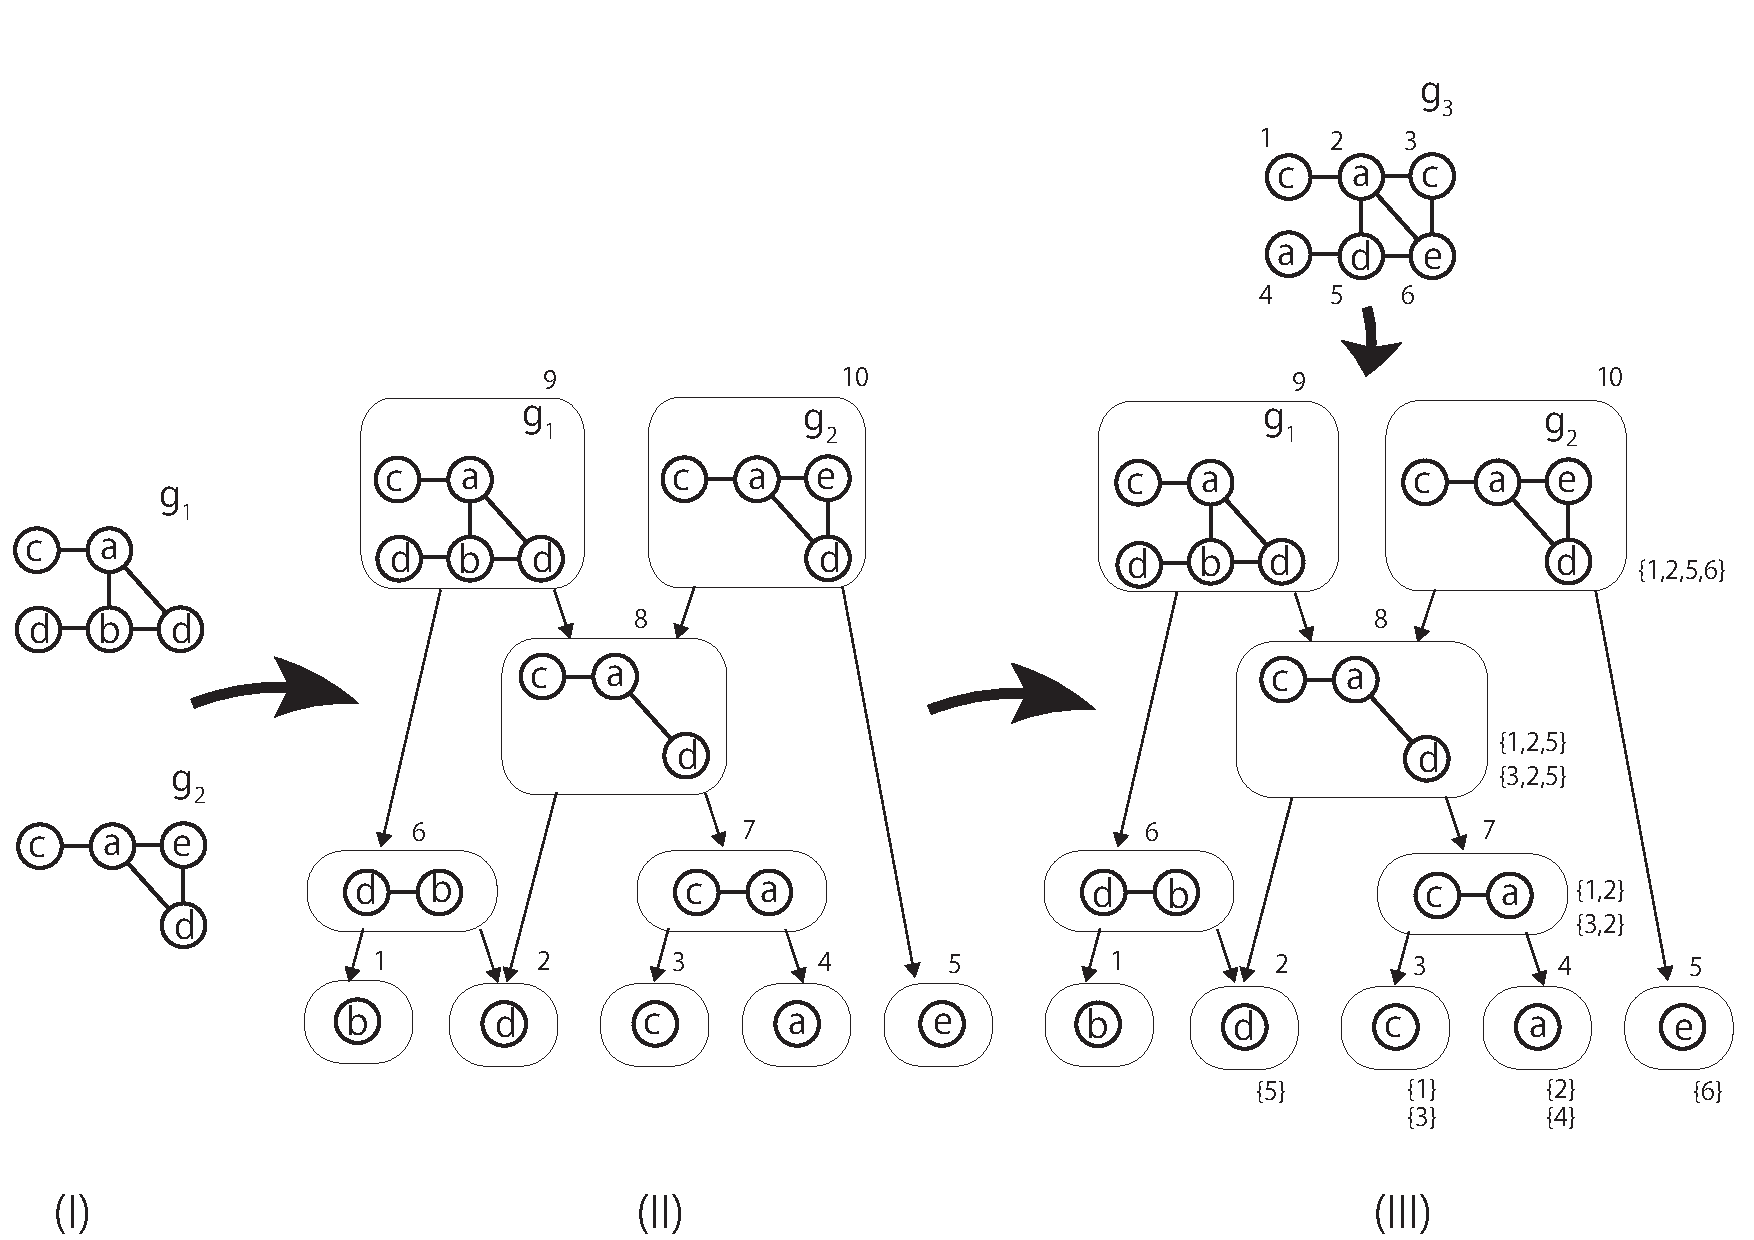
\includegraphics[width=1.0\textwidth]{dag_construction_query_processing6.pdf}
\caption{Schematic of the Network Algorithm: (I) Model Graphs $g_1$ and $g_2$, (II) The Graph Database:A DAG is Constructed using  the model graphs $g_1$ and $g_2$ and their decomposed subgraphs. $DAG$ $node$ $8$ contains a subgraph common to model graphs $g_1$ and $g_2$  (III) Query Processing: Query Graph $g_3$ processed on the Graph Database and the matching query graph node IDs shown in braces}
\label{fig:fig2}
\end{figure}


Messmer et al.\cite{messmer_bunke2000} proposed a so-called \textit{Network Algorithm} to search graphs which are induced subgraphs of a query graph from a graph database. 
A simplified schematic of the algorithm is shown in fig.\ref{fig:fig2}. 
This method also finds all induced subgraph isomorphisms from graphs in the graph database to a query graph.
The \textit{Network Algorithm} consists of two parts.

The first part constructs a directed acyclic graph $DAG$ which stores a set of graphs in a recursively decomposed form.
In the $DAG$,  decomposed graph creation is directed by the original graph and on decomposition 
the directed graph is a \textit{child} and the directing graph is the \text{parent}. 
The left side of Fig.\ref{fig:fig2} shows an example of the decomposition of two model graphs and storing to of the decomposed graph in a database.
Model graphs $g_1$ and $g_2$ are decomposed into two graphs each, in such a way that each pair of decomposed graphs have as close to equal number of vertices  as possible.
Each of the decomposed pair of graphs is further decomposed into two graphs.
This process continues until the decomposition results in singleton graphs.
Before any graph is decomposed, it is checked for containment of an induced subgraph previously created by the decomposition process so far. If one is found, the graph is decomposed into the induced subgraph and a rest subgraph. In this way, an induced subgraph can be shared by multiple parents as shown in Fig.\ref{fig:fig2} where $g_1$ is decomposed randomly into subgraph $6$ and subgraph $8$ by partitioning approximately an equal number of vertices.
If $g_2$ contains an induced subgraph $8$, $g_2$ is decomposed into graph $8$ and graph $5$ after the all decomposition of $g_1$ has finished.

The second part induced subgraph isomorphism query is processed using the $DAG$ constructed in first part.
Initially all induced subgraph isomorphisms from all singleton graphs in the $DAG$ to query graph are detected.
Then, based on the induced subgraph isomorphisms, calculates induced subgraph isomorphisms of the respective parent graphs by combining the induced subgraph isomorphisms of its children. This process repeats until finally, all induced subgraph isomorphisms of model graphs to the query are detected.
The \textit{Network Algorithm} makes use of the fact that if a graph in $DAG$ is not an induced subgraph of query graph, its ancestors are also not induced subgraphs.
In Fig.\ref{fig:fig2} part(III), if \textit{node 8} is not an induced subgraph of $g_3$, we know each of $g_1$ and $g_2$ are also not induced subgraph of $g_3$without performing any additional computation. Using this knowledge the time required to process the induced subgraph query is reduced by avoiding this unnecessary computation. The advantages of the \textit{Network Algorithm}  are:  

\begin{enumerate}
\item The $DAG$ is constructed by decomposing graphs recursively which allows solution of queries by divide and conquer.
\item The induced subgraph isomorphisms of induced subgraphs discovered in the $DAG$ that are common to multiple model graphs are computed only once and the result is shared.
\end{enumerate}

\subsection{Our Contributions}

We propose improvements in two areas: extension of processing to subgraph isomorphism query and more scalable \textit{Network Algorithm}. First, We describe below the improvements to the \textit{Network Algorithm} aimed at more efficient computation of induced subgraph query in the context of induced subgraph query processing. Then we describe the new extensions that enable subgraph query processing. 

%\begin{figure}[t]
%\centering
%\epsfig{file=partition.eps, height=2.3in, width=3in}
%\caption{Two ways to decompose a graph into two subgraphs}
%\label{fig:fig2}
%\end{figure}

\begin{figure}
        \centering
        %& -shell-escape -enable-write18
\documentclass{standalone}
\usepackage{tikz}
\usetikzlibrary{matrix}
\usetikzlibrary{shapes,arrows}
\usepackage{caption}

%\newcommand{mynodename}[#1]{\mathrm{#1}}
%\newcommand{mylabelleft}[#2]{label={[font=\fontsize{#1}{#1}\selectfont]above left:mynodename{#2}}}
\begin{document}

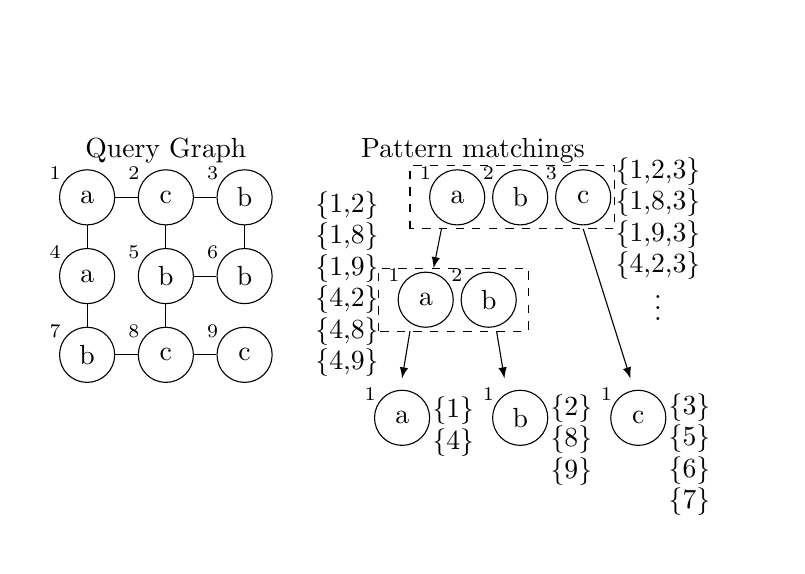
\begin{tikzpicture}[scale=1.0]
%[every node/.style={draw,circle}]
\tikzstyle{every node}=[draw,shape=circle,minimum size=0.7cm];
\tikzstyle{mylabels}=[font=\fontsize{7}{7}\selectfont,yshift=-.2cm];
\tikzstyle{line} = [draw,-latex];
\tikzstyle{dashedline} = [draw,dashed];
\colorlet{invisible}{white}
\colorlet{visible}{black}

\begin{scope}[shift={(.3,.3)}]
%\draw[help lines,step=.2cm] (-1,-6) grid (10,6);;
  \node (n1) at (0,2) [label={[font=\fontsize{7}{7}\selectfont,xshift=.1cm,yshift=-.2cm]above left:$1$}] {a};
  \node (n2) at (1,2) [label={[font=\fontsize{7}{7}\selectfont,xshift=.1cm,yshift=-.2cm]above left:$2$}] {c};
  \node (n3) at (2,2) [label={[font=\fontsize{7}{7}\selectfont,xshift=.1cm,yshift=-.2cm]above left:$3$}] {b};
  \node (n4) at (0,1) [label={[font=\fontsize{7}{7}\selectfont,xshift=.1cm,yshift=-.2cm]above left:$4$}] {a};
  \node (n5) at (1,1) [label={[font=\fontsize{7}{7}\selectfont,xshift=.1cm,yshift=-.2cm]above left:$5$}] {b};
  \node (n6) at (2,1) [label={[font=\fontsize{7}{7}\selectfont,xshift=.1cm,yshift=-.2cm]above left:$6$}] {b};
  \node (n7) at (0,0) [label={[font=\fontsize{7}{7}\selectfont,xshift=.1cm,yshift=-.2cm]above left:$7$}] {b};
  \node (n8) at (1,0) [label={[font=\fontsize{7}{7}\selectfont,xshift=.1cm,yshift=-.2cm]above left:$8$}] {c};
  \node (n9) at (2,0) [label={[font=\fontsize{7}{7}\selectfont,xshift=.1cm,yshift=-.2cm]above left:$9$}] {c};
  
  \node [draw=none] (query_label) at (1,2.6) {Query Graph};% query graph label

  \foreach \from/\to in {n1/n2,n2/n3,n1/n4,n5/n6,n2/n5,n3/n6,n4/n7,n7/n8,n5/n8,n8/n9}
    \draw (\from) -- (\to);
\end{scope}

\begin{scope}[shift={(5,0)}]
	\begin{scope}[shift={(0,0.3)}]%top  row
		\node (n10) at (0,2) [label={[font=\fontsize{7}{7}\selectfont,xshift=.1cm,yshift=-.2cm]above left:$1$}] {a};
		\node (n11) at (.8,2) [label={[font=\fontsize{7}{7}\selectfont,xshift=.1cm,yshift=-.2cm]above left:$2$}] {b};
		\node (n12) at (1.6,2) [label={[font=\fontsize{7}{7}\selectfont,xshift=.1cm,yshift=-.2cm]above left:$3$}] {c};
		\draw[dashedline] (-.6,1.6) rectangle (2,2.4);
		
		\path[line] (-.2,1.6) -- (-.3,1.1);%left side
		\path[line] (1.6,1.6) -- (2.2,-.3);%long arrow on right side

		\node [draw=none] (patternmatching_label) at (.2,2.6) {Pattern matchings};% query graph label
	\end{scope}
	\begin{scope}[shift={(-.4,0)}] %middle row
		\node (n13) at (0,1)  [label={[font=\fontsize{7}{7}\selectfont,xshift=.1cm,yshift=-.2cm]above left:$1$}] {a};
		\node (n14) at (.8,1) [label={[font=\fontsize{7}{7}\selectfont,xshift=.1cm,yshift=-.2cm]above left:$2$}] {b};
		\draw[dashedline] (-.6,.6) rectangle (1.3,1.4);
		\path[line] (-.2,0.6) -- (-.3,0);
		\path[line] (.9,0.6) -- (1,0);
	\end{scope}
	\begin{scope}[shift={(-.7,-.5)}] %bottom row
		\node (n15) at (0,0) [label={[font=\fontsize{7}{7}\selectfont,xshift=.1cm,yshift=-.2cm]above left:$1$}] {a};
		\node (n16) at (1.5,0) [label={[font=\fontsize{7}{7}\selectfont,xshift=.1cm,yshift=-.2cm]above left:$1$}] {b};
		\node (n17) at (3,0) [label={[font=\fontsize{7}{7}\selectfont,xshift=.1cm,yshift=-.2cm]above left:$1$}] {c};
		
	\end{scope}

  \foreach \from/\to in {n1/n2,n2/n3,n1/n4,n5/n6,n2/n5,n3/n6,n4/n7,n7/n8,n5/n8,n8/n9}
    \draw (\from) -- (\to);
\end{scope}
\begin{scope}[shift={(7.5,1.8)}]
			\matrix (m)[matrix of nodes, column  sep=-1mm,color=visible,row  sep=-3mm, anchor=center,draw=none,nodes={rectangle,color=invisible,draw=none}]{ %,text width = 2cm
\node [color=visible] {\{1,2,3\}};&\\
\node[color=visible] {\{1,8,3\}};& \\
\node[color=visible] {\{1,9,3\}};& \\
\node[color=visible] {\{4,2,3\}};& \\
\node[color=visible] {\vdots};& \\
	};
\end{scope}
\begin{scope}[shift={(3.55,1.2)}]
			\matrix (m)[matrix of nodes, column  sep=-1mm,color=visible,row  sep=-3mm, anchor=center,draw=none,nodes={rectangle,color=invisible,draw=none}]{ %,text width = 2cm
\node [color=visible] {\{1,2\}};&\\
\node[color=visible] {\{1,8\}};& \\
\node[color=visible] {\{1,9\}};& \\
\node[color=visible] {\{4,2\}};& \\
\node[color=visible] {\{4,8\}};& \\
\node[color=visible] {\{4,9\}};& \\
	};
\end{scope}
\begin{scope}[shift={(4.9,.2)}]
			\matrix (m)[matrix of nodes, column  sep=-1mm,color=visible,row  sep=-3mm, anchor=north,draw=none,nodes={rectangle,color=invisible,draw=none}]{ %,text width = 2cm
\node [color=visible] {\{1\}};&\\
\node[color=visible] {\{4\}};& \\
	};
\end{scope}
\begin{scope}[shift={(6.4,.2)}]
			\matrix (m)[matrix of nodes, column  sep=-1mm,color=visible,row  sep=-3mm, anchor=north,draw=none,nodes={rectangle,color=invisible,draw=none}]{ %,text width = 2cm
\node [color=visible] {\{2\}};&\\
\node[color=visible] {\{8\}};& \\
\node[color=visible] {\{9\}};& \\
	};
\end{scope}
\begin{scope}[shift={(7.9,.2)}]
			\matrix (m)[matrix of nodes, column  sep=-1mm,color=visible,row  sep=-3mm, anchor=north,draw=none,nodes={rectangle,color=invisible,draw=none}]{ %,text width = 2cm
\node [color=visible] {\{3\}};&\\
\node[color=visible] {\{5\}};& \\
\node[color=visible] {\{6\}};& \\
\node[color=visible] {\{7\}};& \\
	};
\end{scope}
\end{tikzpicture}

\end{document}
        \caption{An example of the explosion of number of matching \label{fig:fig3} }
\end{figure}

\begin{table}
\begin{center}\begin{tabular}{|c|c|c|}
\hline
  & Vertex partition  & Edge partition  \\ \hline
Subgraph & sometimes infeasible  & feasible \\ \hline
Induced subgraph & feasible & sometimes  infeasible \\ \hline
\end{tabular}
\caption{Appropriate method for decompositions \label{tab:table1} }
\end{center}
\end{table}

\begin{figure}
\centering
%& -shell-escape -enable-write18
\documentclass{standalone}
\usepackage{tikz}
%\usepackage{caption}
\usetikzlibrary{external}
\usetikzlibrary{shapes,arrows}
%\newcommand{mynodename}[#1]{\mathrm{#1}}
%\newcommand{mylabelleft}[#2]{label={[font=\fontsize{#1}{#1}\selectfont]above left:mynodename{#2}}}
\begin{document}
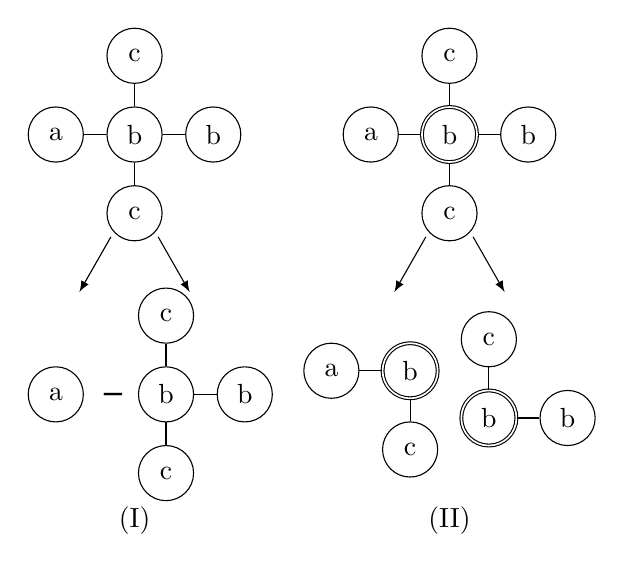
\begin{tikzpicture}[scale=1.0]
%[every node/.style={draw,circle}]
\tikzstyle{every node}=[draw,shape=circle,minimum size=0.7cm];
\tikzstyle{mylabels}=[font=\fontsize{7}{7}\selectfont];
\tikzstyle{line} = [draw,-latex]


%\draw[help lines] (-1.0,-6.0) grid (12.0,6.0);
\begin{scope}[shift={(0,0)}]%upper row set
	\begin{scope}[shift={(1,4.0)}]%upper row left
  		\node (a1) at (0,0) {a};
 		\node (b1) at (1,0) {b};
  		\node (b2) at (2,0) {b};
  		\node (c1) at (1,1) {c};
  		\node (c2) at (1,-1) {c};
  
		\foreach \from/\to in {a1/b1,b1/b2,b1/c1, b1/c2}
   		 \draw (\from) -- (\to);
	\end{scope}
	\begin{scope}[shift={(5.0,4)}]%upper row right
 		 \node (a2) at (0,0) {a};
 		 \node[draw,double,shape=circle,minimum size=0.7cm] (b3) at (1,0) {b};
 		 \node (b4) at (2,0) {b};
		 \node (c3) at (1,1) {c};
 		 \node (c4) at (1,-1) {c};
  
	  	\foreach \from/\to in {a2/b3,b3/b4,b3/c3, b3/c4}
   		 \draw (\from) -- (\to);
	\end{scope}
\end{scope}%upper row set
\begin{scope}[shift={(0,0.7)}]% lower row set
	\begin{scope}[shift={(0,0)}] % lower row extreme left
		\node (a3) at (1,0) {a};
		\node [draw=none] (minus)      at   (1.6,0){\scalebox{2.5}[1.5]{ -} };%horizontal scaling with no vertical scaling
		\node [draw=none] (EdgeCutting) at (2.0,-1.6) { (I) };% edge cutting label
		\node [draw=none] (EdgeCutting) at (6.0,-1.6) { (II) };% edge cutting label
	\end{scope}
	\begin{scope}[shift={(2.4,0)}]%lower row second from left
  		\node (b5) at (0,0) {b};
 		\node (b6) at (1,0) {b};
		\node (c5) at (0,1) {c};
		\node (c6) at (0,-1) {c};
		
		
		\foreach \from/\to in {b5/b6,b5/c5, b5/c6}
			\draw (\from) -- (\to);
	\end{scope}
	\begin{scope}[shift={(4.5,.3)}]% lower row middle right
  		\node (a4) at (0,0) {a};
  		\node[draw,double,shape=circle,minimum size=0.7cm] (b7) at (1,0) {b};
  		\node (c7) at (1,-1) {c};
  
 		 \foreach \from/\to in {a4/b7,b7/c7}
   		 \draw (\from) -- (\to);
	\end{scope}% lower row middle right
	\begin{scope}[shift={(5.5,-.3)}]% lower row extreme right
		\node[draw,double,shape=circle,minimum size=0.7cm] (b8) at (1,0) {b};
		\node (b9) at (2,0) {b};
 		\node (c8) at (1,1) {c};
 	 		\foreach \from/\to in {b8/b9,b8/c8}
	    		\draw (\from) -- (\to);
	\end{scope}% lower row extreme right
\end{scope}%lower row set
\begin{scope}[shift={(0,0)}]% the arrows set
	\begin{scope}[shift={(1.8,2.7)}]%the left arrows
		\path[line] (-0.1,0) -- (-0.5,-0.7);
		\path[line] (0.5,0) -- (0.9,-0.7);
	\end{scope}
	\begin{scope}[shift={(5.8,2.7)}]%the right arrows
		\path[line] (-0.1,0) -- (-0.5,-0.7);
		\path[line] (0.5,0) -- (0.9,-0.7);
	\end{scope}
\end{scope}
\end{tikzpicture}
\end{document}

\caption{Two ways to decompose a graph, (I) \textit{Decomposition to induced subgraph} by partitioning the set vertices (interconnecting edge cutting). (II) \textit{Decomposition to subgraph} by partitioning the set of edges (common vertex sharing).}
\label{fig:fig4}
\end{figure}

\begin{enumerate}
\item Subgraph query processing

\begin{enumerate}

\item Extending the \textit{Network Algorithm} to subgraph query.

The \textit{Network Algorithm} implements only processing of induced subgraph queries. We implement an extension of the method enable processing of subgraph queries. The limitation in the \textit{Network Algorithm} occurs due decomposition by vertex partition used to facilitate induced subgraph isomorphism query. We need to provide a similar facility suited to subgraph isomorphism query. To do so, first we rewrite the algorithms to process subgraphs, mostly by replacing the term \textit{induced subgraph} with \textit{subgraph} in the previous section. Then, we define a new decomposition method by partitioning edges, that is suited for processing subgraphs.


Table. \ref{tab:table1} summarizes feasible approaches to decomposition. In the \textit{Network Algorithm}, graphs are decomposed by cutting edges.
In order to extend the \textit{Network Algorithm} to non-induced subgraph query, we implement \textit{decomposition to subgraph} by partitioning edges (shared vertices). Fig.\ref{fig:fig4} shows the difference between two methods of decomposition. We now describe the rationale for the difference in decomposition described above.

For induced subgraph query, we have to decompose a graph partitioning vertices to form two induced subgraphs and store the information about the interconnecting cut edges. Both the resulting children must be induced subgraphs of their parent to enable the processing of induced subgraph queries in a divide and conquer fashion. However, Decomposing an arbitrary graph into its induced subgraph and rest graph by shared vertices such that both children are induced subgraphs of the parent cannot be assured.

In Fig.\ref{fig:fig51} we see an example where the decomposition of a graph into two induced subgraphs is infeasible by partitioning edges (sharing vertices).
If we decompose $g$ by partitioning edges, the rest graph is $s_{rest}$. But $s_{rest}$ must be induced subgraph of $g$, so the edge is complemented as $s_{rest}'$ and $s_{rest}'$ is equal to $g$. This indicates that we cannot decompose a graph $g$ any further as $g$ is a complete graph.
The subtraction of induced subgraph by partitioning vertices (vertex subtraction)  is defined in \textit{Definition \ref{def:def37}}.

For subgraph query, we need to decompose graphs by partitioning edges. This is due to the requirement that both children must be subgraphs of their parent graphs
and the limitation that we are unable to decompose a graph into an arbitrary subgraph and the rest graph by partitioning vertices so that rest graph becomes subgraph of its parent.
Fig.\ref{fig:fig61} shows an example where a decomposition of a graph into two subgraphs is not feasible by partitioning vertices.
If we subtract $s$ from $g$ by partitioning vertices, $s_{rest}$ cannot be represented as a graph as only an edge remains. We need to subtract the subgraphs by partitioning edges and then including the vertices on the edges as $s_{rest}'$ shows. Hence subgraph query processing we decompose the graphs by partitioning edges and including the corresponding vertices.
The subtraction of subgraphs by partitioning edges (edge subtraction)is defined in \textit{Definition \ref{def:def310}}.

We use the appropriate decomposition for both decompositions and also reform corresponding algorithms.

\item Subgraph processing algorithms

In addition to the specialized routines for subgraph decomposition mentioned in the previous section,  we have also developed a parallel set of routines for both the construction of the $DAG$ and query processing. 

%% Non induced subgraphs can only be decomposed by shared vertices  
\end{enumerate}


\item Induced subgraph query processing

\begin{enumerate}
\item Decomposing a graph into two connected subgraphs.


The \textit{Network Algorithm} decomposes a graph at random and without any restriction on the resulting subgraphs other than that they be connected graphs.
Therefore the decomposition result possibly creates multiple connected graph composed of many small graph fragments.
However the number of matchings from number of smaller graphs to a query graph can easily become intractable.
Fig.\ref{fig:fig3} shows an extreme example of the rapid increase of the matchings that results when a graph is decomposed to singletons.
The number of matchings correlate with processing time as well as memory requirements, hence the need to restrict them. We reformulate the decomposition algorithm with the restriction that a connected graph must be decomposed to strictly result in only two connected subgraphs. When decomposition results in one or both graph disconnected, we post-process the resulting subgraphs by redistributing one or both components between the children  at random until two connected graphs result.

%\begin{figure}
%\centering
%\epsfig{file=images/explosion.eps, height=2.2in, width=3.5in}
%\caption{An example of the explosion of number of matching}
%\label{fig:fig102}
%\end{figure}

\item Early propagation of subgraph search state.

The \textit{Network Algorithm} searches all nodes in $DAG$ from the leaf nodes in a bottom up fashion.
As a result, all the child nodes in the $DAG$ will get processed before the parent nodes. The state of the parent nodes is computed after all the child nodes have been computed. This results in some unnecessary computation in the case that one or more of the children are found not to be isomorphic to a query because a parent graph state determined as non isomorphic if at least one children is not isomorphic to a query.  In fact when the isomorphism state is negative, only one test is sufficient to discover the state of all the ancestral graphs. We use a simple example in Fig.\ref{fig:fig2} (III) to illustrate this.
Assume that we know that $node$ 6 is not a subgraph of query $g_3$ in advance. This implies that $g_1$ is not a subgraph of the query $g_3$.
Hence we need not check $node$ 8 and its descendants to know the status of $g_1$ which we propagate. Further, the potential computation savings increase when a non isomorphic subgraph is common to multiple parents. We propose a recursive algorithm for subgraph search with state propagation of subgraph status to avoid the needless calculations. This results in a \textit{New Network Algorithm} is faster than the \textit{Network Algorithm}.
\end{enumerate}

%\begin{figure}[t]
%\centering
%\epsfig{file=ex_induced_decomposition.eps, height=0.8in, width=3in}
%\caption{An example that a decomposition of a graph into two induced subgraphs is unable by sharing vertices}
%\label{fig:fig11}
%\end{figure}


\begin{figure}
\centering
git%& -shell-escape -enable-write18
\documentclass{standalone}
\usepackage{tikz}
\usetikzlibrary{external}
%\usepackage{caption}
\usetikzlibrary{shapes,arrows}
\newcommand{\mynodelabelfont}[1]{\fontsize{#1pt}{#1pt}\selectfont,yshift=-.2cm}
%\newcommand{mynodename}[#1]{\mathrm{#1}}

\begin{document}
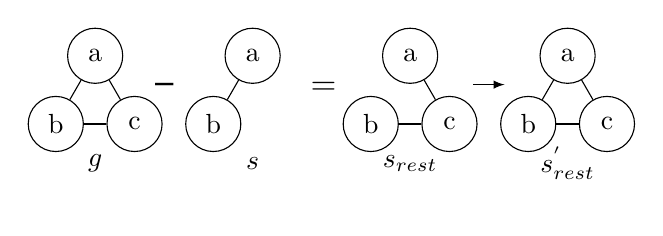
\begin{tikzpicture}[scale=1.0]
%[every node/.style={draw,circle}]
\tikzstyle{myline} = [draw,-latex]
\tikzstyle{every node}=[draw,shape=circle,minimum size=0.7cm];
%\tikzstyle{mylabelsfont=[font=\fontsize{7}{7}\selectfont,yshift=-.2cm];
%\tikzstyle{every label}=[text height=10pt];
\begin{scope}[xshift=0cm]
  \node (a) at (60:1cm) {a};
  \node (b) at (0:0cm)  {b};
  \node (c) at (0:1cm)  {c};
  \node [draw=none] (minus)  at   (1.4,.5){\scalebox{2.5}[1.5]{-} };
  \node [draw=none] (SharedVertices) at (.5,-.5) {$g$};% sharedvertices label


  \foreach \from/\to in {a/b,b/c,c/a}
    \draw (\from) -- (\to);
\end{scope}
\begin{scope}[xshift=2cm]
  \node (a) at (60:1cm) {a};
  \node (b) at (0:0cm)  {b};
  \node [draw=none] (minus)  at   (1.4,.45){\scalebox{1.2}[1.2]{=} };
  \node [draw=none] (SharedVertices) at (.5,-.5) {$s$};%sharedvertices label

  \foreach \from/\to in {a/b}
    \draw (\from) -- (\to);
\end{scope}
\begin{scope}[xshift=4cm]
  \node (a) at (60:1cm) {a};
  \node (b) at (0:0cm)  {b};
  \node (c) at (0:1cm)  {c};
  \node [draw=none] (SharedVertices) at (.5,-.5) {$s_{rest}$};
  \path[myline] (1.3,0.5) -- (1.7,0.5);

  \foreach \from/\to in {b/c,c/a}
    \draw (\from) -- (\to);
\end{scope}
\begin{scope}[xshift=6cm]
  \node (a) at (60:1cm) {a};
  \node (b) at (0:0cm)  {b};
  \node (c) at (0:1cm)  {c};
  \node [draw=none] (SharedVertices) at (.5,-.5) {$s_{rest}^{'}$};

  \foreach \from/\to in {a/b,b/c,c/a}
    \draw (\from) -- (\to);
\end{scope}

\end{tikzpicture}
\end{document}

\caption{A case where decomposition of induced subgraph by partitioning edges (shared vertices) is not feasible \label{fig:fig51} }
\end{figure}

%% Induced graphs can only be decomposed by edge cutting 
%\begin{figure}[t]
%\centering
%\epsfig{file=ex_typical_decomposition.eps, height=0.8in, width=3in}
%\caption{An example that a decomposition of a graph into two subgraphs is unable by cutting edges}
%\label{fig:fig10}
%\end{figure}

\begin{figure}
\centering
%& -shell-escape -enable-write18
\documentclass{standalone}
\usepackage{tikz}
\usetikzlibrary{external}
%\usepackage{caption}
\usetikzlibrary{shapes,arrows}

\newcommand{\mynodelabelfont}[1]{\fontsize{#1pt}{#1pt}\selectfont,yshift=-.2cm}

\begin{document}
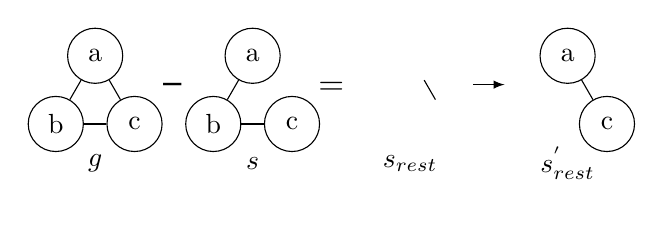
\begin{tikzpicture}[scale=1.0]
%[every node/.style={draw,circle}]
\tikzstyle{line} = [draw,-latex]
\tikzstyle{every node}=[draw,shape=circle,minimum size=0.7cm];
\colorlet{invisible}{white}
\colorlet{visible}{black}
%\tikzstyle{every label}=[text height=10pt];
\begin{scope}[xshift=0cm]
%\draw[help lines] (-1,-6) grid (10,6);
  \node (a) at (60:1cm) {a};
  \node (b) at (0:0cm)  {b};
  \node (c) at (0:1cm)  {c};
  	 \node [draw=none] (minus)  at   (1.5,.5){\scalebox{2.5}[1.5]{-} };
  	 \node [draw=none] (EdgeCutting) at (.5,-.5) {$g$};% edge cutting label

  \foreach \from/\to in {a/b,b/c,c/a}
    \draw (\from) -- (\to);
\end{scope}
\begin{scope}[xshift=2cm]
  \node (a) at (60:1cm) {a};
  \node (b) at (0:0cm)  {b};
   \node (c) at (0:1cm)  {c};
     \node [draw=none] (minus)  at   (1.5,.45){\scalebox{1.2}[1.2]{=} };
 	 \node [draw=none] (EdgeCutting) at (.5,-.5) {$s$};%sharedvertices label
  
  \foreach \from/\to in {a/b,b/c}
    \draw (\from) -- (\to);
\end{scope}
\begin{scope}[xshift=4cm]
  \node[color=invisible] (a) at (60:1cm) {a};
  \node[color=invisible] (c) at (0:1cm)  {c};
    \node [draw=none] (EdgeCutting) at (.5,-.5) {$s_{rest}$};
    \path[line] (1.3,0.5) -- (1.7,0.5);

  \foreach \from/\to in {a/c}
    \draw (\from) -- (\to);
\end{scope}
\begin{scope}[xshift=6cm]
  \node (a) at (60:1cm) {a};
  \node (c) at (0:1cm)  {c};
  \node [draw=none] (EdgeCutting) at (.5,-.5) {$s_{rest}^{'}$};

  \foreach \from/\to in {c/a}
    \draw (\from) -- (\to);
\end{scope}
\end{tikzpicture}

\end{document}

\caption{A case where decomposition of subgraph by partitioning vertices (cutting edges) is not feasible \label{fig:fig61} }
\end{figure}

\begin{figure}
\centering
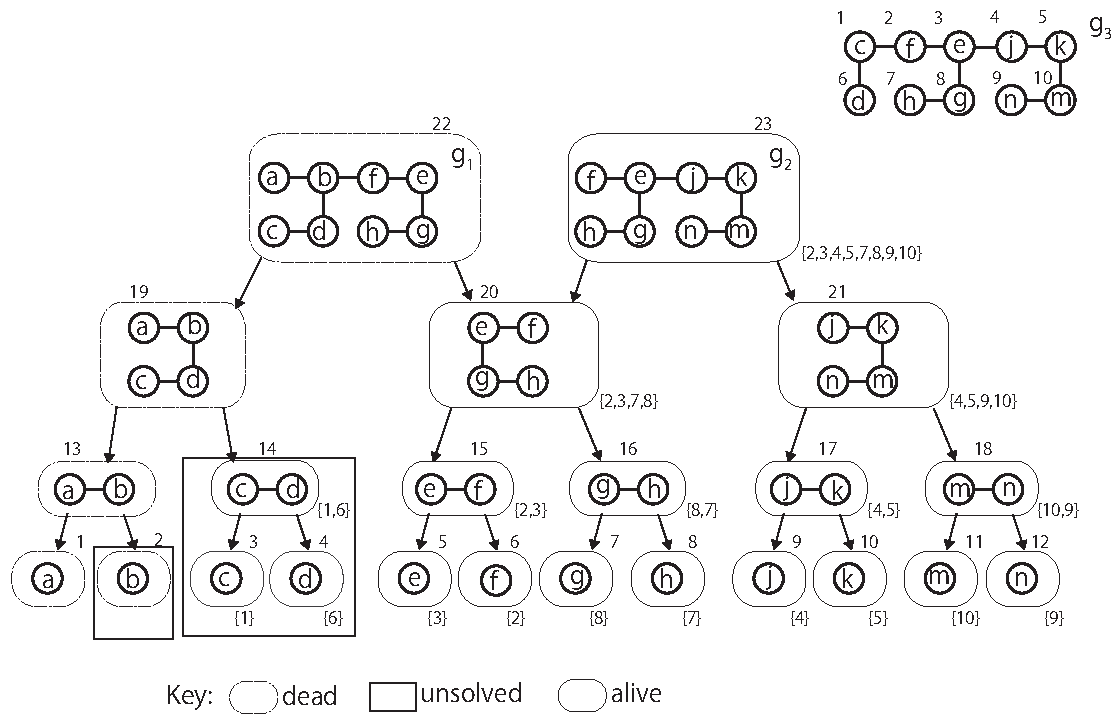
\includegraphics[width=1.0\textwidth]{dag_search_optimize.pdf}
\caption{The search strategy for the \textit{New Network Algorithm}: For a simplified database composed of model graphs $g_1$ and $g_2$, given a query graph $g_3$ each model graph is processed locally by starting at the top of the $DAG$ in a depth first search (DFS) fashion. The search concludes when the first \textit{dead} state is encountered. Specifically, we conclude that nodes 1,13,19, 22 (hence model graph $g_1$) are in \textit{dead} state as soon as node 1 is processed. After processing $g_1$ and $g_2$ we have the result in spite of nodes 2,3,4, and 14 remaining in \textit{unsolved} state. In contrast, the \textit{Network Algorithm} processes \textit{all} the nodes in the $DAG$ in the order of the numbers on the top right of the nodes before any output is delivered.}
\label{fig:fig7}
\end{figure}


\section{Proposed Algorithms}
In this section, we present details for the proposed \textit{ New Network algorithm} and related algorithms. 
There are two main contributions: a new faster search strategy and extension to processing of subgraph queries.
Further, we also describe in detail the improved algorithms for processing of induced subgraph query.

%We now describe the algorithms for processing subgraph query and induced subgraph query in detail.

As an  overview, the algorithms solve two problems, database creation and query processing. Accordingly we divide the discussion into them into two corresponding parts.
The first part is concerned with the construction of a dynamic acyclic graph $DAG$ to store the model graphs. 
The model graphs are stored in a network with their decomposed subgraphs and the related links and state information. 
Specifically, we construct a $DAG$ consisting of a set of 5-Tuples, each of which  stores information about a graph, its state, its parents, its children and the Edges connecting the pair of child graphs. 
Creation of the DAG is performed by recursively decomposing the Model graphs and creating a 5-tuple for each resulting graph to store the information. 
The 5-tuples can be considered as nodes in the DAG as they are connected by a directed edge from parent to child.

The second group of Algorithms concerns the process of detecting subgraph isomorphisms using $DAG$ constructed in previous part. 
The $DAG$ is the central data structure for this work and is considered  a global variant in all the algorithms. 

\subsection{DAG definition}
First we make a formal definition to help us write the algorithms for the DAG more concisely.


Let $G=\{g_1 ,\ldots, g_n \}$ be a set of model graph. 
\begin{definition}
A \emph{DAG}  $D(G)$  is a finite set of 5-tuple ($g,s,P,C,E$) constructed by decomposition of a set of model graphs $G$ where $g$ is a graph, $s$ is one of $\{unsolved, dead, alive\}$,  $P$ is a set of one or more parent graphs $\{p^{'},p^{''}\ldots \}$ , $C$ is a set of two child graphs $\{c^{'},c^{''}\}$ of graph $g$, and $E$ is a set of edges connecting the child graphs $c{'}$ and $c^{''}$. 
The $DAG$ has to satisfy the following conditions.


\begin{enumerate}[(1)]
%\item $g$ and $c^{'} ,c^{''} $ are graphs with $c^{'}\subset g$ and $c^{''} \subset g$.
\item  $c^{'}\subset g$ and $c^{''} \subset g$ for each child  $c^{'},c^{''}$ of graph $g$
\item  $g \subset p^{'}$, $g \subset p^{''} \ldots$, for each parent in $p$ of graph $g$
%\item $E$ is a set of edges such that $g=c^{'}\cup_{E} c^{''}$
\item $g=c^{'}\cup_{E} c^{''}$
%\item For each $g_{i}$ in $G$ there exists a $5-tuple$ ($g,s,P,C,E$) $\in$ $D(G)$ 
\item For each $g_{i}$ in $G$ there exists a $5-tuple$ ($g,s,P,C,E$) $\in$ $D(G)$ 
\item For each  $5-tuple$ ($g,s,P,C,E$) $\in$ $D(G)$ there exists no other  $5-tuple$ ($g,s,P,C,E$) $\in$ $D(G)$ with $g=g_1$.
\item For each  $5-tuple$ ($g,s,P,C,E$) $\in$ $D(G)$

\begin{enumerate}[a.]
\item if $c^{'},c^{''} \in C$  consist of graphs with more than one vertex, then there exists a corresponding pair of  $5-tuple$ 
\item if $c^{'},c^{''} \in C$ consist of one vertex then there exists no corresponding $5-tuple$ 
\end{enumerate}

\end{enumerate}
\end{definition}

\begin{definition}
A graph $g$ is disconnected if its vertex set $V$ can be partitioned into two nonempty, disjoint subsets $V_1$ and $V_2$ such that there exists no edge in $g$ whose one end is in subset $V_1$ and the other end is in subset $V_2$
\end{definition}

\begin{definition}
The size of a graph $g$ is defined as $|V| + |E|$, the sum of the number of Vertices and Edges  in the graph, and is denoted by $|g|$. 
\end{definition}  

\begin{definition}
The \textit{minimal component} of a disconnected graph $g$ is defined as a  disjoint component graph of a disconnected graph such that no other disjoint component has fewer vertices.
The \text{minimal component} of disconnected graph $g$ is denoted by $g_{min}$.
\end{definition}  


\subsection{Expansion to Subgraph Isomorphism Query with reduced search space}

The method of graph decomposition used in the \textit{Network Algorithm} is restricted in its  support to induced subgraph isomorphism query processing only. 
However, in practice,  subgraph isomorphism query is more likely to suit real world problems therefore we reformulate the \textit{Network Algorithm} to process subgraph isomorphism query. 
In this subsection, we describe the details of the expansion of the \textit{Network Algorithm} to allow subgraph query processing and also propose some addition improvements. 
Some of our improvements applied to subgraph query are also applicable to induced subgraph queries which is addressed in the next subsection. For these algorithms, we use parenthesis such as (induced) subgraph to separate the two cases. 
We first discuss the subgraph isomorphism so ignore the inside of the parentheses throughout this subsection.

\subsubsection{DAG Construction}
The $DAG$ is the main data structure for the database construction and query processing. 
In this section we outline the steps required to construct the $DAG$ as well as the use of the $DAG$ to process queries. 
First the algorithm for the construction of the DAG is show in Algorithm \ref{alg:alg01} below.


\begin{algorithm}
\caption{createDAG(G)}
\label{alg:alg01}
\begin{algorithmic}
\STATE Input: Model Graphs $G =\{g_1,g_2,\dots,g_m\}$
\STATE Output: $D(G)= \{$($g,s,P,C,E$)$,\ldots,$($g_n,s_n,P_n,C_n,E_n$)$ \}$
\end{algorithmic}
\begin{algorithmic}[1]
\STATE Initialize DAG, $D:=\emptyset$
\FOR{ $i=1$ to $m$}
 \STATE  $\emph{D} \leftarrow $createTuples($g_i,D$)
\ENDFOR
\RETURN $\emph{D(G)}$
\end{algorithmic}
\end{algorithm}

\begin{algorithm}
\caption{CreateTuples($g,D$)} 
\label{alg:alg02}
\begin{algorithmic}
\STATE Input: Connected, non-singleton Graph $g$, Current DAG $D$
\STATE Output: DAG with current tuples and new tuples from graph $g$ added, $D^{'}$
\end{algorithmic}
\begin{algorithmic}[1]
%%\STATE $P = \cup_{i=1}^n \{g_i ,g_i^{'},g_i^{''} \}$ where n is the number of Model graphs in DAG
%\STATE Graph set $g \leftarrow \emptyset$
\STATE Isomorphic graph set $Z \leftarrow \emptyset$
\STATE graph $ z  \leftarrow \emptyset $
\STATE Default node state $s  \leftarrow unsolved$
\STATE Set of Parent Graphs, $P \leftarrow \emptyset$
\STATE Local DAG initialized with current tuples $D^{'} \leftarrow D$

\FOR{each Tuple $\{(z,s_{z} ,P_{z},\{c^{'}, c^{''}\},E)\}  \in D^{'}$ where vertex count $|z| \leq |g|$}
%\STATE let $z$ be the current graph in DAG
\IF{ graph $z$ is $\subseteq_{(induced)} g$}
\STATE Add graph $z$ to $Z$ 
% \STATE $Z$ $\leftarrow$  SubgraphQuery$(DAGIndexGraph, g)$
\ENDIF
\ENDFOR
\WHILE{$Z\neq \emptyset$} 
\IF{$z=g$}
\STATE $P_{z} \leftarrow P_{g}$
%\STATE let $z$ be a child of $g$'s parents $P_g$ and delete $g$
\STATE $D^{'} \leftarrow D^{'} \cup \{(z,s,P_z ,\{\emptyset \} ,\emptyset)\}$
\RETURN $D^{'}$
\ELSE
\FOR{each graph $z$ in $Z$}
\STATE \ $z_{rest}  \leftarrow  (g -_{(induced)} z)$
\IF{$z_{rest}$ is connected}
%\STATE Let \emph{$z_{rest}$} be a child of \emph{$g$}
\STATE $D^{'}  \leftarrow D^{'} \cup \{(g,s_{g},P_g,\{ \emptyset \} , \emptyset )\}$
\STATE $D^{'}  \leftarrow D^{'} \cup \{(z_{rest},s_{z_{rest}},\{g\},\{\emptyset \} , \emptyset )\}$
\STATE CreateTuples($z_{rest}$)
\RETURN  $D^{'}$
\ENDIF
\ENDFOR
\ENDIF
\ENDWHILE
%\IF{ $g$ is not a singleton graph}
%\IF{$g$ is connected}
\STATE  $(g,s_{g},\emptyset,\{z,z_{rest}\},E) \leftarrow RandomPartition(g,s_{g},\emptyset,\{\emptyset \}, \emptyset )$
%\ELSE
%\STATE distribute the components of $g$ to $z$ and $z_{rest}$, with common Edges $E$
%\ENDIF
%\STATE let $z$ and $z_{rest}$ be the children of $g$
\STATE $D^{'}  \leftarrow D^{'} \cup \{(g,s_{g},\emptyset,\{z,z_{rest}\},E)\}$
\STATE $D^{'}  \leftarrow D^{'} \cup \{(z,s_{z},\{g\},\{ \emptyset \}, \emptyset )\}$
\STATE $D^{'}  \leftarrow D^{'} \cup \{(z_{rest},s_{z_{rest}},\{g\}, \{ \emptyset \} , \emptyset )\}$
\STATE CreateTuples($z$)
\STATE CreateTuples($z_{rest}$) 
%\ENDIF
\RETURN $D^{'}$
\end{algorithmic}
\end{algorithm}


\begin{algorithm}
\caption{ConnectGraph($g,s,P,\{c^{'},c^{''}\},E$)}
\label{alg:alg03}
\begin{algorithmic}
\STATE Input: graph with disconnected childgraphs ($g,s,P,\{c^{'},c^{''}\},E$)
\STATE Output: graph with connected childgraphs ($g,s,P,\{c^{'},c^{''}\},E$)
\end{algorithmic}
\begin{algorithmic}[1]
\STATE $c^{'} \leftarrow  \emptyset $ 
\STATE $c^{''} \leftarrow  \emptyset $ 
\IF{ graph $g$ has a single edge e($v_1$,$v_2$)}
   \STATE Insert $v_{1}$ to $c^{'}, v_{2}$ to $c^{''}$
\ELSE 
\REPEAT
%%\STATE $E_{c^{'}} \leftarrow \emptyset $
%%\STATE $E_{c^{''}} \leftarrow \emptyset $
	\IF{ $c^{'}$ \AND $c^{''}$ are disconnected}
             \IF{ $|c^{'}| > |c^{''}|$ }
                  \STATE $  c^{''} \leftarrow c^{''} \cup  c^{'}_{min} $
             \ELSE
                \STATE $  c^{'} \leftarrow c^{'} \cup c^{''}_{min} $
%%              \STATE $min \{c^{'} , c^{''} \} \leftarrow min \{c^{'} , c^{''} \} \cup $ minimal component of $max\{c^{'} , c^{''} \}$ 
%%		\STATE select larger graph from $\{c^{'} , c^{''} \}$ 
%%              \STATE move minimal component to opposite graph
             \ENDIF
        \ELSE
                \IF { $c^{'}$ is disconnected}
                   \STATE $  c^{''} \leftarrow c^{''} \cup c^{'}_{min} $
%                  \STATE select disconnected graph from $\{c^{'} , c^{''} \}$
%                  \STATE move minimal component to opposite graph
                \ELSE
                   \STATE $  c^{'} \leftarrow c^{'} \cup c^{''}_{min}$ 
                \ENDIF
        \ENDIF
%%	\STATE reset edges induced by distributed vertices to $c^{'}$ and $c^{''}$ 

\UNTIL{ $c^{'}$ \AND $c^{''}$ are connected}
%% \WHILE{ $c^{'}$ or $c^{''}$ not connected}
%%  \IF{ both $c^{'}$ \AND $c^{''}$ are disconnected}
%%    \STATE select graph $|c^{'},c^{''}|_{max}$
%%    \STATE move minimum component to $|c^{'},c^{''}|_{min}$
%%  \ELSE
%%    \STATE select disconnected component from $\{c^{'} , c^{''} \}$
%%    \STATE move component of disconnected graph to opposite $c$
%%  \ENDIF

%% \ENDWHILE
\ENDIF
\RETURN ($g,s,P,\{c^{'},c^{''}\},E$)
\end{algorithmic}
\end{algorithm}


\begin{algorithm}
\caption{RandomPartition($g,s,P,\{c^{'},c^{''}\},E$)}
\label{alg:alg04}
\begin{algorithmic}
\STATE Input: graph $g$
\STATE Output: ($g,s,P,\{c^{'},c^{''}\},E$) is a 5-tuple consisting of graph $g$, a state $s$ children $\{c^{'},c^{''}\}$  and a set of edges between the children $E$ 
\end{algorithmic}
\begin{algorithmic}[1]
\IF{ $g$ has a single edge $e=(v_1,v_2)$}
    \STATE   $c^{'} \leftarrow \{v_1 \}$
    \STATE   $c^{''} \leftarrow \{v_2 \}$    
 \ELSE
   \STATE ($g,s,P,\{c^{'},c^{''}\},E$) $\leftarrow$ RandomPartitionInduced($g,s,P,\{\emptyset \},E$)
\ENDIF
\RETURN ($g,s,P,\{c^{'},c^{''}\},E$)
\end{algorithmic}
\end{algorithm}


\begin{algorithm}
\caption{New Network Algorithm, NNA($D , q$)}
\label{alg:alg05}
\begin{algorithmic}
\STATE Input: Model graphs in DAG, $D(G)= \{$($g_1 ,s_1 ,P_1 ,\{c^{'}_1 ,c^{''}_1 \},E$)$,\ldots,$($g_n,s_n,P_n,\{c_n^{'},c_n^{''}\},E_n$)$ \}$, Query $q$
\STATE and the set of all subgraphs in DAG, $G_{all} = \cup_{i=1}^n \{g_1 ,c_1^{'},c_1^{''},g_2 ,c_2^{'},c_2^{''}\ldots \}$ 
\STATE Output: $Z$, the set of all subgraph isomorphisms in Model graphs in $D$ to query $q$ 
\end{algorithmic}
\begin{algorithmic}[1]
\STATE $F \leftarrow \emptyset$
\STATE $Z \leftarrow \emptyset$
%%\FOR{ each $(g,s,P,\{c^{'},c^{''}\}) \in  D$}
\FOR{ each subgraph in $G_{all}$}
  \STATE  $s \leftarrow unsolved$
\ENDFOR
\FOR{ each $(g,s,P,\{c^{'},c^{''}\}) \in D$}
   \STATE $F \leftarrow $SubgraphQuery($g,s,P,\{c^{'},c^{''}\},q$)
   \IF{$F\neq \emptyset$}
      \STATE $Z \leftarrow Z \cup \{F\}$
   \ENDIF
\ENDFOR
\RETURN $Z$
\end{algorithmic}
\end{algorithm}


\begin{algorithm}
\caption{SubgraphQuery$(g,s,P,\{c^{'},c^{''}\},E, q)$}
\label{alg:aalg06}
\begin{algorithmic}
\STATE Input: Model graph 5-Tuple ($g,s,P,\{c^{'},c^{''}\},E$), query $q$
\STATE Output: Induced Subgraph Isomorphisms, $F$
\end{algorithmic}
\begin{algorithmic}[1]
%%\STATE $F \leftarrow \emptyset $
\IF{ $s$ = $unsolved$ }
\STATE $F \leftarrow \emptyset $
    \IF{ $g$ is a singleton }
        \STATE $F \leftarrow$ AssignVertex($g$,$q$)
      \ELSE 
        %% \STATE let $c^{'}$, $c^{''}$ be children of $g$
         \IF{  $s_{c^{'}}  = dead$ \OR $s_{c^{''}} = dead$}
          \STATE  $s \leftarrow dead$
          \RETURN $F$
          \ELSIF{SubgraphQuery$(c^{'} ,s_{c^{'}} ,P_{c^{'}} ,\{c^{'}_1 ,c^{''}_1 \},E_1 ,q) = \emptyset$ \\ \OR SubgraphQuery$(c^{''} ,s_{c^{''}} ,P_{c^{''}} ,\{c^{'}_2 ,c^{''}_2 \},E_2 ,q) = \emptyset$}
			\STATE $s \leftarrow dead$
                         \RETURN $F$
		\ELSE
			\STATE $F \leftarrow$ CombineInduced$(g,s,P,\{c^{'},c^{''}\},E ,q)$
		\ENDIF
	\ENDIF
	\IF{$F \neq \emptyset$}
		\STATE $s \leftarrow alive$
	\ELSE
		\STATE $s \leftarrow dead$
                 \RETURN $F$
	\ENDIF
\ELSE
%%	\STATE $F$ is the already calculated subgraph isomorphisms from $g$ to $q$
        \RETURN $F$
\ENDIF
%%\RETURN $F$
          
\end{algorithmic}
\end{algorithm}


CreateTuples(Algorithm\ref{alg:alg02}) outlines the dynamic tuple insertion algorithm for $DAG$. 
In order to construct $DAG$ with model graphs , we first decompose the model graphs. 
Then we create and insert the corresponding 5-tuples and the into the $DAG$ to form a graph database. 
Model graphs are inserted in the $DAG$ sequentially.

In constructing the $DAG$, as a rule, each graph in a tuple directs two (induced) subgraphs. 
The exception being that $g$ will have no children if $g$ is a singleton graph. 
The information about the shared vertices in the children and the mappings between a parent and children is  stored with a parent-child relationship in the 5-tuple.

First, the algorithm searches all (induced) subgraphs of $g_i$ in $DAG$(line 6-10). 
For this (induced) subgraph search, SubgraphQuery (Algorithm \ref{alg:aalg06}) explained in the latter section is used. 
The discovered (induced) subgraphs are inserted to a queue $Z$.

If we find that a graph $z$ in $Z$ is isomorphic to $g_i$, we replace the graph by setting a directed edge from the parent of $g_i$ to $z$ (line 12-15).
The existence of graph isomorphism is easily ensured by checking whether $E(g_i)$ is equals to $E(z)$ or not. 
In most cases, a (induced) subgraph $z$ of $g_i$ will be discovered. 
In that case, the algorithm calculates $z_{rest} = g_i -_{(induced)} z$ and $g_i$ is decomposed into the $z$ and the rest graph $z_{rest}$.
If $z_{rest}$ is connected, $z_{rest}$ is inserted to $DAG$ recursively(line 17-25).
There is the case that $z_{rest}$ is disconnected, which is a violation of the requirement that a connected graph is decomposed into two connected graphs. 
When faced with this violation the algorithm abandons the result and tests the subtractions of all (induced) subgraph isomorphisms of all (induced) subgraphs until $z_{rest}$ becomes connected.

The order in which the  (induced) subgraph are tested for subtraction relies ordering of the graph in $Z$.
We know that The larger a graph is, the more costly it is to compute the (induced) subgraph isomorphisms therefore we sort $Z$ to make larger graphs precede to ensure larger subgraphs are shared.

If no (induced) subgraph is discovered or no (induced) subgraph can make $z_{rest}$ connected, $g_i$ is decomposed by the RandomPartition (Algorithm\ref{alg:alg04}).
The decomposed (induced) subgraphs are inserted to $DAG$ recursively(line 38-33).
%In the case that $g_i$ is disconnected, $g_i$ is decomposed by distributing its components to two children so that decomposed graphs finally become connected graphs(line 33-35).

The \textit{Network Algorithm} decomposes a graph by distributing vertices randomly and creating subgraphs which are induced by the distributed vertices.
This decomposition may create disconnected subgraphs composed of many tiny components.
Conceivably, the number of matchings resulting from a large number of such disconnected graphs to a query graph can easily skyrocket hence need to make sure that the decomposed subgraphs are connected to avoid this problem. Effectively, the \textit{Network Algorithm} decomposes a graph by partitioning vertices for induced subgraph query

We now focus on processing of subgraphs which are not induced. In this case, the subtraction of an arbitrary subgraph from a graph requires the decomposition of a graph by partitioning edges.

RandomPartition (Algorithm\ref{alg:alg04}) decomposes a connected graph $g$ into two connected subgraphs.
First, the algorithm distributes edges at random to form two graphs. If at least one subgraph is disconnected, the two subgraphs transfer their minimal components to the opposite side. 
This movement of components likely results in connected graphs because the parent graph $g$ is connected.
The transfer of components is repeated until both subgraphs become connected. 

The limit for decomposing a graph comes when there is a single edge, which we cannot decompose further by partitioning vertices. 
Hence, RandomPartition algorithm cannot process a singleton graph or a disconnected graph which includes one or more isolated vertices. 
To overcome this limitation, we decompose a single edge by partitioning vertices.

%% \begin{algorithm}
%% \caption{RandomPartition($g$)}
%% \label{alg:alg07}
%% \begin{algorithmic}
%% \STATE Input: Graph $g$
%% \STATE Output: A pair of graphs $(s_1, s_2)$
%% \end{algorithmic}
%% \begin{algorithmic}[1]
%% \STATE let $s_1 := \emptyset$, $s_2 := \emptyset$
%% \IF{$g$ is composed of a single edge $e = (v_1, v_2)$}
%% 	\STATE insert $v_1,v_2$ to $s_1,s_2$ respectively
%% \ELSE
%% 	\STATE $(s_1, s_2)$ RandomPartitionInduced($g$)
%% 	\WHILE{either $s_1$ or $s_2$ is disconnected}
%% 		\IF{both $s_1$ and $s_2$ is disconnected}
%% 			\STATE select graph $|s_{1} ,s_{2} |_{max}$
%%                         \STATE move minimum component to opposite side
%% 		\ELSE
%% 			\STATE select disconnected graph from $\{s_1 , s_2 \}$
%%                         \STATE move minimum component to opposite side
%% 		\ENDIF
%% 	\ENDWHILE
%% \ENDIF
%% \RETURN $(s_1,s_2)$
%% \end{algorithmic}
%% \end{algorithm}

\subsubsection{Query Processing}
There are two types of query processing to the graph database; induced subgraph query and the subgraph query. 
In this section we outline the algorithms and discuss both types of processing.
The \textit{New Network Algorithm} (Algorithm \ref{alg:alg05}) outlines the procedure for the (induced) subgraph isomorphism query processing.
Using the SubgraphQuery (Algorithm \ref{alg:aalg06}) we can calculate the (induced) subgraph isomorphism of any graph stored in a node in $DAG$ to a query graph $q$.
We evaluate (induced) subgraph isomorphism query by processing SubgraphQuery with all model graphs as input.

In the procedure for the (induced) subgraph search, all nodes in $DAG$ are set to one of three states using tags, $alive$, $dead$ or $unsolved$.
Those tags indicate three states:(a) already matched  with the query graph and (induced) subgraph isomorphisms exists, (b) already matched and (induced) subgraph isomorphism does not exist, (c) not been matched yet respectively. Initially, all nodes in $DAG$ are tagged $unsolved$.

SubgraphQuery processes the decomposed input graph in the $DAG$ in a recursive manner.
If the input graph $g$ is already tagged $alive$ or $dead$, there is nothing to do and the algorithm only returns subgraph isomorphism $F$  already calculated.

If $g$ is a singleton graph there are no child graphs so SubgraphQuery calls AssignVertex(Algorithm\ref{alg:alg07}) to simply search the occurrences of the label of the single vertex in a query graph $q$.

If $g$ marked $unsolved$, we check (induced) subgraph isomorphism of its children by calling SubgraphQuery recursively.
We exploit the knowledge that if a child is not a (induced) subgraph of a query graph, its parent cannot be a (induced) subgraph of the query graph.
First, in order to avoid unnecessary isomorphism computation we check the tags of children of $g$ before we call SubgraphQuery. 
Next, we call SubgraphQuery for $g$'s children. If at least one child tagged $dead$ or returns an empty set, we are can tag $g$ as $dead$.  
Only in the case that both of the children are tagged with or return the state $alive$ do we have to calculate the (induced) subgraph isomorphisms from $g$ to $q$.

To process the query $q$, we can use already computed child graph's (induced) subgraph isomorphism to $q$ to reduce the computational effort of 
calculating (induced) subgraph isomorphism from $g$ to $q$. For this purpose, a procedure for combining of induced subgraph isomorphisms is required.

Combine (Algorithm\ref{alg:alg08}) is the procedure for the combining subgraph isomorphisms. When Combine is called with $g$ as input, the subgraph 
isomorphisms $F_1, F_2$ from its children $c^{'}, c^{''}$ to $q$ are supposed to be already computed.
In the case that $g$ is connected, two conditions must be satisfied to combine two functions, $f_1 \in F_1, f_2 \in F_2$.
First, it we must ensure that each corresponding common vertices is mapped correctly onto same vertex (line 11).
Second, the image of non-common vertices of $f_1$ and $f_2$ must be disjoint (line 12).
Satisfaction of these conditions ensures that the combining of $f_1$ and $f_2$ is injective.
If $g$ is disconnected, we only need to check one condition that the images of $f_1$ and $f_2$ are disjoint (line 20).
We define the combination of (induced) subgraph isomorphisms as follows
\begin{eqnarray}
\label{eq:eq1}
f(v) = \left\{
\begin{array}{l}
f_1(\bar{p_1}(v)) \quad \bar{p_1}(v) \in V_{c^{'}}\\
f_2(\bar{p_2}(v)) \quad \bar{p_2}(v) \in V_{c^{''}}
\end{array}
\right.
\end{eqnarray}
 
Where $\bar{p_1}$ and $\bar{p_2}$ are functions from parent graph $g$ to childgraphs $c^{'}$ and $c^{''}$ respectively.
The Combine algorithm checks all pairs of functions $f_1$ and $f_2$ and when a pair is found that satisfies these conditions, the algorithm evaluates and returns it.

However this algorithm is limited to graphs decomposable by partitioning edges such that if a graph consisting of a single edge
is input, the Combine algorithm has to call Combineinduced (Algorithm\ref{alg:alg010}) which is able to process graphs decomposable by partitioning vertices..

\begin{algorithm}
\caption{AssignVertex($g,q$)}
\label{alg:alg07}
\begin{algorithmic}
\STATE Input: Singleton graph $g=(V,E,L^v ,L^e ,\mu,\nu)$, Query graph $q=(V_q,E_q,L_q^v ,L_q^e ,\mu_q,\nu_q)$ 
\STATE Output: Subgraph isomorphisms $F$
\end{algorithmic}
\begin{algorithmic}[1]
\STATE $F \leftarrow \emptyset$
\STATE let $v \in V$
\FOR{each $v_q \in V_q$}
	\IF{$\mu(v)= \mu_q (v_q)$}
		\STATE add $f(v) = v_q$ to $F$
	\ENDIF
\ENDFOR
\RETURN $F$
\end{algorithmic}
\end{algorithm}

\begin{algorithm}
\caption{Combine$(g,s,P,\{c^{'},c^{''}\},E, q)$}
\label{alg:alg08}
\begin{algorithmic}
\STATE Input: Graph 5-Tuple $(g,s,P,\{c^{'},c^{''}\},E)$, Query graph $q$
\STATE Output: Subgraph isomorphisms $F$
\end{algorithmic}
\begin{algorithmic}[1]
\IF{$g$ is composed of a single edge}
	\STATE $F \leftarrow$ CombineInduced$(g,s,P,\{c^{'},c^{''}\},E, q)$
\ELSE
%%	\STATE let $c^{'}$ and $c^{''}$ be children of $g$
        \STATE $F_1 \leftarrow$ Combine$(c^{'} , s_{c^{'}} , P_{c^{'}} , \{c^{'}_1 ,c^{''}_1 \},E_1 , q)$
        \STATE $F_2 \leftarrow$ Combine$(c^{''} ,s_{c^{''}} ,P_{c^{''}} ,\{c^{'}_2 ,c^{''}_2 \},E_2 , q)$
%%	\STATE let $p_1$ and $p_2$ be functions from $g$ to $c^{'}$ and $c^{''}$
%%	\STATE let $F_1$ and $F_2$ be sets of injection from $c^{'}$ and $c^{''}$ to query graph
	\STATE $F \leftarrow \emptyset$
	\IF{$g$ is connected}
		\STATE $V_c = V_g - (V_1 \cup V_2) $ 
		\FOR{each pair ($f_1, f_2$) in ($F_1, F_2$) }
			\IF{$f_1(\bar{p_1}(V_c)) = f_2(\bar{p_2}(V_c))$}
				\IF{$f_1(V_{c^{'}}) \cap f_2(V_{c^{''}}) = f_1( \bar{p_1}(V_c) )$}
%%					\STATE define subgraph isomorphism $f$ by eq(\ref{eq:eq1})
                                        \STATE $g \leftarrow (c^{'} \cup_{E} c^{''})$
                                        \STATE $V_g \leftarrow f(V_{c^{'}} \cup V_{c^{''}} })$
                                        \STATE $F \leftarrow  F \cup \{ f \} $
				\ENDIF
			\ENDIF
		\ENDFOR
	\ELSE
		\FOR{each $f_1 \in F_1, f_2 \in F_2$}
			\IF{$f_1(V_{c^{'}}) \cap f_2(V_{c^{''}}) = \emptyset$}
%%				\STATE define subgraph isomorphism $f$ by eq(\ref{eq:eq1})
                                \STATE $g \leftarrow (c^{'} \cup_{E} c^{''})$
                                \STATE $V_g \leftarrow f(V_{c^{'}} \cup V_{c^{''}} })$
                                \STATE $F \leftarrow  F \cup \{ f \} $
			\ENDIF
		\ENDFOR
	\ENDIF
\ENDIF
\RETURN $F$
\end{algorithmic}
\end{algorithm}

%\subsection{Expansion to Subgraph Isomorphism Query with Improvements}
%The method of graph decomposition used in the \textit{Network Algorithm} restricts its  support to induced subgraph isomorphism query only. However, in practice,  subgraph isomorphism query is more likely to suit real world problems therefore we reformulate the \textit{Network Algorithm} to process subgraph isomorphism query. In this subsection, we describe the details of the expansion of the \textit{Network Algorithm} to allow subgraph query processing and also propose some addition improvements. Some of our improvements applied to induced subgraph query are also applicable to subgraph queries which was addressed in the previous subsection. We first discuss the subgraph isomorphism so ignore the inside of the parentheses throughout this subsection.

\subsection{Induced Subgraph Query}
The improvement algorithms proposed in previous subsection are also efficient for induced subgraph query.
In this subsection, we explain the detail algorithms for our induced subgraph query processing.
Many of algorithms of induced subgraph query are same as that of subgraph query, therefore when we reference the 
previous subsection, take the insides of the parenthesises into consideration to indicate the induced versions.

\subsubsection{DAG Construction}
The procedure for the construction of $DAG$ and dynamic insertion algorithm are also almost identical to the case of subgraph query.
We now explain the differences. First, a parent-child relationship must store the information about the edges between partitioned vertices instead of the vertices common graphs. 
This is due of the difference in the manner of decomposition of the graphs. 
Second, the existence of a graph isomorphism is assured by checking whether input graph $V(g_i)$ is equal to a graph $V(s)$ in the DAG or not.

In order to decompose an arbitrary graph into two smaller induced subgraphs we have to decompose a graph by partitioning vertices hence we define a procedure for decomposing a randomly connected graph in this manner.

RandomPartitionInduced (Algorithm\ref{alg:alg09}) decomposes a connected graph into two connected induced subgraphs.
First, the algorithm initializes two induced subgraphs by distributed vertices and the edges that the vertices induce.
Then, two subgraphs transfer their minimum components until they become connected, a process similar to the one in the algorithm for subgraph query.

The decomposition of a disconnected graph is identical to the one for subgraph query.

\begin{algorithm}
\caption{RandomPartitionInduced}
\label{alg:alg09}
\begin{algorithmic}
\STATE Input: 5-Tuple of Graph $(g,s,P,\{c^{'},c^{''}\},E)$
\STATE Output: 5-Tuple of a pair of graphs $(c^{'},s,P_1 ,\{c^{'}_1 ,c^{''}_1 \},E_1 )$, $(c^{''},s,P_2 ,\{c^{'}_2 ,c^{''}_2 \},E_2 )$
\end{algorithmic}
\begin{algorithmic}[1]
\STATE  $c^{'} \leftarrow  \emptyset$
\STATE  $c^{''} \leftarrow \emptyset$
\STATE  $s_1 \leftarrow s$
\STATE  $s_2 \leftarrow s$
%%\STATE  $\{V_{c^{'}} , V_{c^{''}}\} \leftarrow V_g $ 
%%\STATE  partition at random $V_g $ to $V_{c^{'}}$ and $V_{c^{''}}$
%%\STATE $| V_{c^{'}} | = | V_g / 2 |$
%%\STATE $| V_{c^{''}} | = | V_g | - | V_{c^{'}} |$
\WHILE {$|V_{c^{'}}| \leq   \lfloor |V_g |/2 \rfloor $} \DO
       \STATE $v \leftarrow$ random vertex of $ V_g $
       \STATE $V_{c^{'}} \leftarrow V_{c^{'}} \cup v $ 
       \STATE  $ V_g \leftarrow V_g - v $
\ENDWHILE
\STATE $ V_{c^{''}} \leftarrow V_g $
\STATE  $E_{c^{'}} \leftarrow $ Edges induced in $V_{c^{'}}$ by $g $
\STATE  $E_{c^{''}} \leftarrow $ Edges induced in $V_{c^{''}}$ by $g$
\STATE  $c^{'} \leftarrow \{V_{c^{'}} , E_{c^{'}}  \}$ 
\STATE  $c^{''} \leftarrow \{V_{c^{''}} , E_{c^{''}}  \}$ 
%%\STATE $E_1 \leftarrow  E \cap ( E_{c^{'}} \cup E_{c^{''}} )$
%%\STATE $E_2 \leftarrow  E \cap ( E_{c^{'}} \cup E_{c^{''}} )$
%%\STATE $P_1 \leftarrow \{g\}$
%%\STATE $P_2 \leftarrow \{g\}$
\REPEAT
%%\STATE $E_{c^{'}} \leftarrow \emptyset $
%%\STATE $E_{c^{''}} \leftarrow \emptyset $
	\IF{ $c^{'}$ \AND $c^{''}$ are disconnected}
             \IF{ $|c^{'}| > |c^{''}|$ }
                  \STATE $  c^{''} \leftarrow c^{''} \cup  c^{'}_{min} $
             \ELSE
                \STATE $  c^{'} \leftarrow c^{'} \cup c^{''}_{min} $
%%              \STATE $min \{c^{'} , c^{''} \} \leftarrow min \{c^{'} , c^{''} \} \cup $ minimal component of $max\{c^{'} , c^{''} \}$ 
%%		\STATE select larger graph from $\{c^{'} , c^{''} \}$ 
%%              \STATE move minimal component to opposite graph
             \ENDIF
        \ELSE
                \IF { $c^{'}$ is disconnected}
                   \STATE $  c^{''} \leftarrow c^{''} \cup c^{'}_{min} $
%                  \STATE select disconnected graph from $\{c^{'} , c^{''} \}$
%                  \STATE move minimal component to opposite graph
                \ELSE
                   \STATE $  c^{'} \leftarrow c^{'} \cup c^{''}_{min}$ 
                \ENDIF
        \ENDIF
%%	\STATE reset edges induced by distributed vertices to $c^{'}$ and $c^{''}$ 

\UNTIL{ $c^{'}$ \AND $c^{''}$ are connected}
\STATE $E_1 \leftarrow  E -  ( E_{c^{'}} \cup E_{c^{''}} )$
\STATE $E_2 \leftarrow  E -  ( E_{c^{'}} \cup E_{c^{''}} )$
\STATE $P_1 \leftarrow \{g\}$
\STATE $P_2 \leftarrow \{g\}$
\RETURN  ($(c^{'},s,P,\{c^{'}_1 ,c^{''}_1 \},E_1 )$, $(c^{''},s,P,\{c^{'}_2 ,c^{''}_2 \},E_2 )$)
\end{algorithmic}
\end{algorithm}

\subsubsection{Query Processing}
The search processing algorithms for subgraphs, \textit{NNA} (Algorithm\ref{alg:alg05}), SubgraphQuery (Algorithm\ref{alg:aalg06}) and AssignVertex(Algorithm\ref{alg:alg07}) are also applicable to induced subgraph query. However, due to the difference in the method of decomposition, we need a new procedure for the combining the 
induced subgraph isomorphisms. CombineInduced(Algorithm\ref{alg:alg010}) outlines that procedure.
When CombineInduced is called with graph $g$ as input, the sets of induced subgraph isomorphisms $F_1, F_2$ from its children $c^{'}, c^{''}$ 
to the query graph must have been already calculated, as part recursive calling of \label{alg:aalg06}.
There are two conditions that must be satisfied to CombineInduced two functions $f_1 \in F_1 and f_2 \in F_2$.
First, there must exist edges in the query graph correspond to cut edges and vice versa(line 7).
Second, we must ensure that $f_1$ and $f_2$ are disjoint(line 8), otherwise the combination of $f_1$ and $f_2$ will not be injective function.
CombineInduced algorithm checks all pairs of the two functions and returns the sets of its unions that satisfy these conditions.

\begin{algorithm}[t]
\caption{CombineInduced}
\label{alg:alg010}
\begin{algorithmic}
\STATE Input:  Graph 5-Tuple $(g,s,P,\{c^{'},c^{''}\},E)$, Query graph $q$
\STATE Output: Subgraph isomorphisms $F$
\end{algorithmic}
\begin{algorithmic}[1]
%%\STATE let $c^{'}$ and $c^{''}$ be children of $g$
%%\STATE let $\bar{p_1}$ and $\bar{p_2}$ be functions from $g$ to $c^{'}$ and $c^{''}$
%%\STATE let $F_1$ and $F_2$ be sets of injection from $c^{'}$ and $c^{''}$ to query graph
\STATE $F_1 \leftarrow$CombineInduced$(c^{'},s_1 ,P_1 ,\{c_1^{'},c_1^{''}\},E_1 ,q)$
\STATE $F_2 \leftarrow$CombineInduced$(c^{''},s_2 ,P_2 ,\{c_2^{'},c_2^{''}\},E_2 ,q)$
\STATE $F \leftarrow \emptyset$
\STATE $E \leftarrow E_g - (E_1 \cup E_2 )$
\FOR{each pair $(f_1, f_2 )$ in $(F_1, F_2 )$}
		\IF{ for each $e = (v_1, v_2) \in E$ there exists  $e_q = (f_1(v_1),f_2(v_2)) \in E_q$ with $\nu(e) = \nu_q(e_q)$ 
\STATE \AND for each $e_q = (u_1, u_2) \in E_q$ such that $u_1 \in f_1(V_{c^{'}}), u_2 \in  f_2(V_{c^{''}}) $ there exists $e = (f_1^{-1}(u_1), f_2^{-1}(u_2)) \in E$ with $\nu_q(e_q) = \nu(e)$}	
			\IF{$f_1(V_{c^{'}}) \cap f_2(V_{c^{''}}) = \emptyset$}
                                \STATE $g \leftarrow (c^{'} \cup_{E} c^{''})$
                                \STATE $V_{g} \leftarrow f(V_{c^{'}} \cup V_{c^{''}} })$
                                \STATE $F \leftarrow  F \cup \{ f \} $
%%				\STATE define subgraph isomorphism $f$ by eq(\ref{eq:eq1})
%%				\STATE $F = F \cup f $
		\ENDIF
	\ENDIF
\ENDFOR
\RETURN $F$
\end{algorithmic}
\end{algorithm}

\subsection{Network Algorithm with Graph Pruning}
The \textit{Network Algorithm} cannot process a local query efficiently (i.e. In the case that you want to know subgraph isomorphisms for only some graphs in a graph database to a query graph, the \textit{Network Algorithm} calculates subgraph isomorphisms for all the nodes in $DAG$).
In contrast our recursive formulation of the \textit{Network Algorithm} only checks the relevant descendants of selected nodes and this allows us to solve local queries more efficiently.

One result of the support of local query is that we can make use of some graph pruning techniques. Let us consider a simple example \textit{label check}. 
If a graph database stores the numeric labels of attributed graphs, it may be easily determined when they have no subgraph isomorphisms to a query graph just by comparing the attributes of the graph with those of the query graph.
In this way, we can efficiently reduce the candidates graphs for the answer.
Consequently, by pruning graphs in advance, we can significantly reduce the related procesing time.


% LocalWords:  EdgeIDs


\section{Performance and Evaluation}

\subsection{Experimental Setup}
The source code was developed in the C++ language and compiled using Microsoft Visual Studio 2010 Ultimate. The hardware consisted of a Dell T1500 personal computer with an
Intel Core i-3 CPU 3.09 GHZ, 16 Gbyte memory, running the Windows 7 Professional Operating system.

\subsection{The Datasets}

Two types datasets are used in the experiments. The first type is the synthetic dataset of Erd\"{o}s-R\`{e}nyi random graphs. The parameters used to generate the synthetic dataset are shown in table \ref{tab:parameterTable}. Different sets of both query graphs and database were generated for each instance of Edge density and Label count. The result is 8 sets of random Graph Query-Database pairs. The query graph size varies from 10 vertices to 80 vertices, with either 5 or 10 vertex labels. The database graph has 10 vertices, with either 5 or 10 vertex labels. The database graph count varies from 1000 graphs to 20000 graphs. We also generated an one sparse query-database set for experiments to replicate the dataset of Messmer et. al \cite{messmer_bunke2000}. for the purpose of comparative evaluation of their algorithm which proved to be an order of magnitude or more slower on regular random graphs for even moderate increases in query graph size beyond 10 vertices and 12 edges.

The second type is the real dataset, that is generated from AIDS Antiviral Screen data. This data contains around 43,000 chemical compounds and is available publicly from NCI \footnote{National Cancer Institute http://dtp.nci.nih.gov/}. The graphs created from the antiviral compounds data, is denoted `` AIDS'' and has on average, 25 vertices and 27 edges. The maximum is 438 vertices and 441 edges. There are 63 distinct vertex labels and 3 distinct edge labels.

The random decomposition affects the processing time such that each individual run is different even for an identical query and database set. To minimize this we processed each query exactly 10 times over the database and averaged processing time.

\subsection{Synthetic Data}


\begin{table}
\begin{center}
\begin{tabular}{|l|l|r|r|r|c|r|r|r|r|}  \hline
\multirow{3}{*}{Experiment} & \multicolumn{5}{c|}{Database} & \multicolumn{4}{c|}{Query}  \\ \cline{2-2} \cline{3-3} \cline{4-4} \cline{5-5} \cline{6-6} \cline{7-7} \cline{8-8} \cline{9-9} \cline{10-10}
       & \multicolumn{2}{c|}{Vertices} & \multicolumn{2}{c|}{Edges} & Graphs & \multicolumn{2}{c|}{Vertices} & \multicolumn{2}{c|}{Edges} \\ \cline{2-2} \cline{3-3} \cline{4-4} \cline{5-5}  \cline{7-7} \cline{8-8} \cline{9-9} \cline{10-10} 
 & \#  & Labels & \# & Labels &  & \#  & Label & \# & Labels  \\ \hline
Fig 9 & 10 & 10 & 26\% & 1 & 100 $\sim$ 20K & 10 & 10 & 26\% & 1 \\ \hline
  & 10 & 10 & 50\% & 1 & 100 $\sim$ 20K & 10 & 10 & 50\% & 1 \\ \hline
 & 10 & 10 & 75\% & 1 & 100 $\sim$ 20K & 10 & 10 & 75\% & 1 \\ \hline
 & 10 & 10 & 100\% & 1 & 100 $\sim$  20K & 10 & 10 & 100\% & 1 \\ \hline
 & 10 & 5 & 26\% & 1 & 100 $\sim$  20K & 10 & 5 & 26\% & 1 \\ \hline
 & 10 & 5 & 50\% & 1 & 100 $\sim$  20K & 10 & 5 & 50\% & 1 \\ \hline
 & 10 & 5 & 75\% & 1 & 100 $\sim$  20K & 10 & 5 & 75\% & 1 \\ \hline
 & 10 & 5 & 100\% & 1 & 100 $\sim$ 20K & 10 & 5 & 100\% & 1 \\ \hline
\end{tabular}
\caption{ Synthetic Graph Generation Parameters \label{tab:parameterTable} }
\end{center}
\end{table}


We test the performance of our algorithm with regard to induced subgraph query by evaluating the proposed algorithm and comparing it with Messmer's Network Algorithm and the state-of-the-art sequential scan algorithm for subgraph isomorphism, VF2\cite{cordella2001_vf2}. We also evaluate our algorithm with regard to non-induced subgraph query, where we compare proposed algorithm with the sequential scan(VF2) only.


\subsubsection{The Effect of size of Query and Database graph size on  the processing time}
The graphs in Figure\ref{fig:fig91} show the effect of Query and Database size on processing time.  


\begin{figure}[H]
\centering
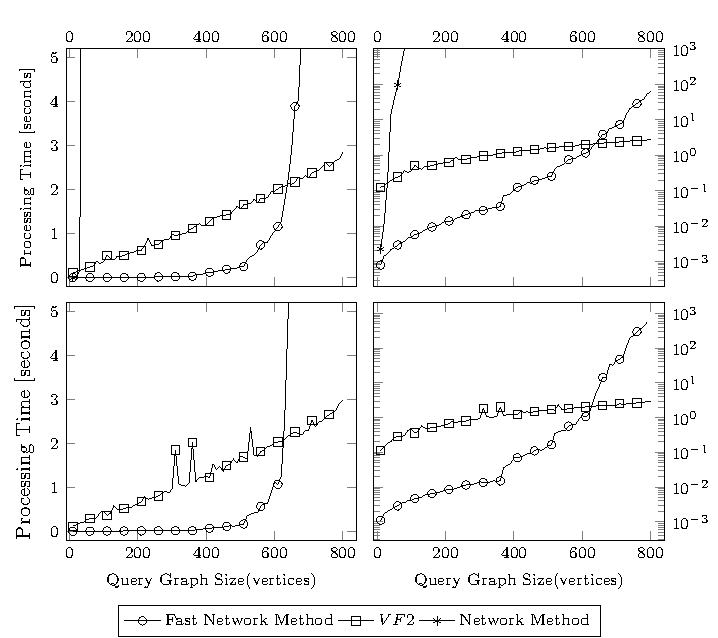
\includegraphics[width=1.0\textwidth]{syndataplot.pdf}
\caption{\textbf{Effect of Query Graph Size on Processing Time of Synthetic Graphs} 

\texttt{(a)} Linear and \texttt{(b)} Linear-log plot of \textit{induced subgraph} query processing time against query graph size. \texttt{(c)} Linear and \texttt{(d)} Linear-log plot of \textit{subgraph} query processing time for increasing size of graph query.
}
\label{fig:fig91}
\end{figure}

Fig\ref{fig:fig91} \texttt{(a).} Shows a linear plot of induced subgraph query processing time against query graph vertex count. The query graph size ranges from 10 vertices to 800 vertices. The \textit{Fast Network Method} and the \textit{Network Method} are faster for subgraph queries of up to about 600 vertices. For larger query graphs, the \textit{VF2} method is faster. The \textit{Network Method} takes more than 5sec for induced subgraph query graph larger than 10 vertices. The \textit{VF2} method shows an almost linear time dependency of query graph vertex count, an advantage for induced subgraph queries larger than 600 vertices. 

Fig\ref{fig:fig91} \texttt{(b).} Shows a linear-log plot of the induce subgraph graph query processing time with query graph size. We observe that for induced subgraph query size less than 400 Vertices, there is an order of magnitude or better advantage to the \textit{Fast Network Method}. Beyond query graphs of about 600 vertices the \textit{VF2} method is clearly superior. We observe that the \textit{Network Method} is slowest, taking about 15min for an induced subgraph query of just 80 vertices.

Fig\ref{fig:fig91} \texttt{(c).} Shows a linear plot of  query processing time for increasing size of graph query.The smallest query graph contains 10 vertices while the largest query graph contains 800 vertices. The \textit{Fast Network Method} processes query graphs faster than \textit{VF2} for subgraphs not larger than 600 vertices. Here too, \textit{VF2} method shows an almost linear processing time  dependency with query graph size.  

Fig\ref{fig:fig91} \texttt{(d).} Shows a linear-log plot of the induce subgraph graph query processing time with query graph size. For subgraph query size less than about 400 Vertices, there is an order of magnitude or better advantage to the \textit{Fast Network Method}. For synthetic graphs of less that 50 vertices, the advantage is about two orders of magnitude. Beyond query graphs of about 600 vertices the \textit{VF2} method is superior.



\subsubsection{Effect of number of graphs in the Query and Database on the processing time}

\begin{figure}[H]
\centering
\includegraphics[width=1.0\textwidth]{syndata_graphcount.pdf}
\caption{\textbf{Effect of Graph Count on Processing Time of Synthetic Graphs}} 
\label{fig:graphcount}
\end{figure}



\subsubsection{Effect of Number of Labels in Query and Database Graphs on processing time}

\begin{figure}[H]
\centering
\includegraphics[width=1.0\textwidth]{syndata_labels.pdf}
\caption{\textbf{Effect of Labels on Processing Time of Synthetic Graphs}}
\label{fig:labels}
\end{figure}


\subsubsection{Effect of Number of Edge Density in Query and Database Graphs on processing time}

\begin{figure}[H]
\centering
\includegraphics[width=1.0\textwidth]{syndata_edgedensity.pdf}
\caption{\textbf{Effect of Edge Density on Processing Time of Synthetic Graphs}} 
\label{fig:edgedensity}
\end{figure}





\subsection{Real Data}

\subsubsection{Effect of size of query and Database graph count on processing time}

\begin{figure}[H]
\centering
\includegraphics[width=1.0\textwidth]{realdataplot.pdf}
\caption{\textbf{Effect of Query Size on Processing Time of Real World Graphs} 


\textbf{ Top left:}Linear-linear plot of  induced subgraph query processing time for increasing size of query graph.The smallest query graph contains 10 vertices while the largest query graph contains 60 vertices. The \textit{Fast Network Method} and the textit{Network Method} show almost identical processing times. The \textit{VF2} method is noticably slower. 


\textbf{Top Right:} Linear-log plot of the induce subgraph graph query processing time with query graph size. The \textit{Fast Network Method} and the textit{Network Method} are almost indistinguishable and show an order of magnitude advantage over the state-of-the-art \textit{VF2} Method 

\textbf{ Bottom left:}Linear-linear plot of  query processing time for increasing size of graph query. The smallest query graph contains 10 vertices while the largest query graph contains 60 vertices. The \textit{Fast Network Method} is faster than \textit{VF2} for subgraphs as well. The \textit{VF2} method takes more than 50s to process query graphs large than 10 vertices. 

\textbf{Bottom Right:} Linear-log plot of the graph query processing time with query graph size. Both the \textit{Fast Network Method} and the textit{Network Method} are almost indistinguishable and show more than an order of magnitude advantage over the \textit{VF2} Method.}

\label{fig:fig81}
\end{figure}



\subsection{Graph Database Processing}

\begin{figure}[H]
\centering
\includegraphics[width=1.0\textwidth]{syndata_database.pdf}
\caption{\textbf{Results of the Experiments on the Synthetic Graph Data Set}}
\label{fig:database}
\end{figure}

END

In this section we perform experiments on two datasets to evaluate the performance of the new algorithm in practice.

In this section, we evaluate the proposed algorithms on two datasets and compare the results to two well known graph isomorphism detection algorithms. The first dataset is a set of synthetic graphs. These are aggregated in of several graph databases featuring one of several fixed edge densities, label counts and total database graph count. We call his the synthetic dataset. The second dataset is  a set of graphs modeling active ingredients in antiviral drugs for the treatment of AIDS. We call this the AIDS dataset. 

We perform tests to evaluate the effect of several dataset parameters on the processing time.
We perform two sets of tests; In the first set, we evaluate our algorithms on the retrieval of induced subgraph to query and In the second set, we evaluate retrieval of non induced sugraph to query.

To test the efficacy of our algorithm with regard to induced subgraph query, we evaluate the proposed algorithm in comparison with Messmer's Network Algorithm and a sequential SCAN using the state-of-the-art subgraph isomorphism detection algorithm VF2\cite{cordella2001_vf2}.
We also evaluate our algorithm with regard to non-induced subgraph query, where we compare proposed algorithm with the sequential scan only.
All the algorithms were implemented using the C++ programming language and run on a Intel Core i-3 CPU 3.09 Ghz, 16 Gbyte memory, Personal Computer running Windows 7 Professional Operating system.

\subsection{Graph Datasets}
We evaluate our algorithms by processing the retrieval of descriptors from the compounds dataset.
We use AIDS Antiviral Screen dataset to provide a real graph dataset.
This dataset contains around 43,000 chemical compounds and is available publicly from NCI
\footnote{National Cancer Institute http://dtp.nci.nih.gov/}.
We denote this dataset as ``AIDS'' in our experiment.
The graphs of AIDS have an average number of 25 vertices and 27 edges, a maximum of 438 vertices and 441 edges,
63 distinct vertex labels and 3 distinct edge labels.

In order to evaluate our algorithms over a larger database to test scalability, we use synthetic large dataset. 
The graph generator is configured to emit only connected graphs thathave an edge probability of 50 percent. 
Except where explicitly stated, 10 distinct vertex labels and 10 distinct.

\begin{figure}[h]
\centering
\includegraphics[width=1.0\textwidth]{images/realdataplot.pdf}
\caption{\textbf{Results of the Experiments on the Real World Graph Data Set} 


\textbf{ Top left:}Linear-linear plot of  induced subgraph query processing time for increasing size of query graph.The smallest query graph contains 10 vertices while the largest query graph contains 60 vertices. The \textit{Fast Network Method} and the textit{Network Method} show almost identical processing times. The \textit{VF2} method is noticably slower. 


\textbf{Top Right:} Linear-log plot of the induce subgraph graph query processing time with query graph size. The \textit{Fast Network Method} and the textit{Network Method} are almost indistinguishable and show an order of magnitude advantage over the state-of-the-art \textit{VF2} Method 

\textbf{ Bottom left:}Linear-linear plot of  query processing time for increasing size of graph query. The smallest query graph contains 10 vertices while the largest query graph contains 60 vertices. The \textit{Fast Network Method} is faster than \textit{VF2} for subgraphs as well. The \textit{VF2} method takes more than 50s to process query graphs large than 10 vertices. 

\textbf{Bottom Right:} Linear-log plot of the graph query processing time with query graph size. Both the \textit{Fast Network Method} and the textit{Network Method} are almost indistinguishable and show more than an order of magnitude advantage over the \textit{VF2} Method.}

\label{fig:fig81}
\end{figure}

\subsection{Chemical Descriptor Search}
In chemistry, substructures of compounds that imply a chemical, physical property of the compound are called as descriptor.
Fast retrievals of descriptors from compounds aids research of compounds.
We evaluate our algorihm by processing the retrievals of descriptors.
We builded a model graph database $D$ by extracting graph database $W$ composed of 10,000 compounds whose size are less than 40 from AIDS and applying frequent graph mining to $W$.
We set minimum support as 5 percent.
$D$ is composed of 18930 distinct frequent subgraphs.

We vary average size of query graphs and evaluate query processing time.
For each plot, 100 query graphs are extracted from $W$.
Query processing time is time to process the all query graphs and the time to construct the DAG is excluded. In the results we compare the processing time of two methods with our proposed \textit{Fast Network Algorithm}. These methods are: 

The \textit{Network algorithm}, in which the use of $DAG$ data structure to store the graphs was pioneered. This method however was only implemented for induced subgraph queries, so we are only able to perform comparisons for half of the experiments. 

The state-of-the-art one-on-one graph query algorithm \textit{VF2}. This algorithm  tests a graph for subgraph isomorphism or induced subgraph isomorphism to another single graph only. This is repeated sequentially for a large graph database. The solution is a binary true or false answer. It cannot be used to find all isomorphisms to a graph in a database as one is not able to differentiate multiple isomorphisms from a binary response.

We now analyse the results.

The  top left of Fig.\ref{fig:fig81} shows a Linear-linear plot of induced subgraph query processing time for increasing size of query graph. In this experiment, the smallest query graph contains 10 vertices while the largest query graph contains 60 vertices. For this real world graph database the \textit{Fast Network Method} and the textit{Network Method} show almost identical processing times. In this evaluation \textit{VF2} method is the slowest, taking more than 50 seconds to process query graphs containing more than 10 vertices. The fact that the \textit{Fast Network Method} is not substantially better than the \textit{network Method} implies that we do not have many fragmented graphs during decomposition, hence there is no advantage in ensuring that all decomposed graphs are connected.  

Top Right of Fig.\ref{fig:fig81} shows a Linear-log plot of the induce subgraph graph query processing time with query graph size. We observe that both the \textit{Fast Network Method} and the textit{Network Method}, while almost indistinguishable, show an order of magnitude advantage in processing time over the state-of-the-art \textit{VF2} Method. 

Bottom left of Fig.\ref{fig:fig81} shows a Linear-linear plot of  query processing time with increasing  time in the  graph query. The experiment was performed using query graphs containing 10 vertices to 60 vertices. Here \textit{Fast Network Method} is faster than \textit{VF2} for subgraphs too. We also observe that the \textit{VF2} method takes more than 50s to process query graphs large than 10 vertices. 

Bottom Right of Fig.\ref{fig:fig81} shows a Linear-log plot of the graph query processing time with increasing query graph size. We observe that both the \textit{Fast Network Method} and the \textit{Network Method} while almost indistinguishable, show more than an order of magnitude advantage in processing time over the state-of-the-art \textit{VF2} Method.

It is because that their are originally few decompositions that creates disconnected graphs and also few redundant subgraph isomorphism detections in DAG.
So in this experiment, our improvements did not work.

Fig.\ref{fig:fig4} shows the processing time for subgraph isomorphism query.
Fig.\ref{fig:fig4} indicates the subgraph isomorphism query is faster than SCAN same as Messmer et al's algorithm.

\begin{figure}[h]
\centering
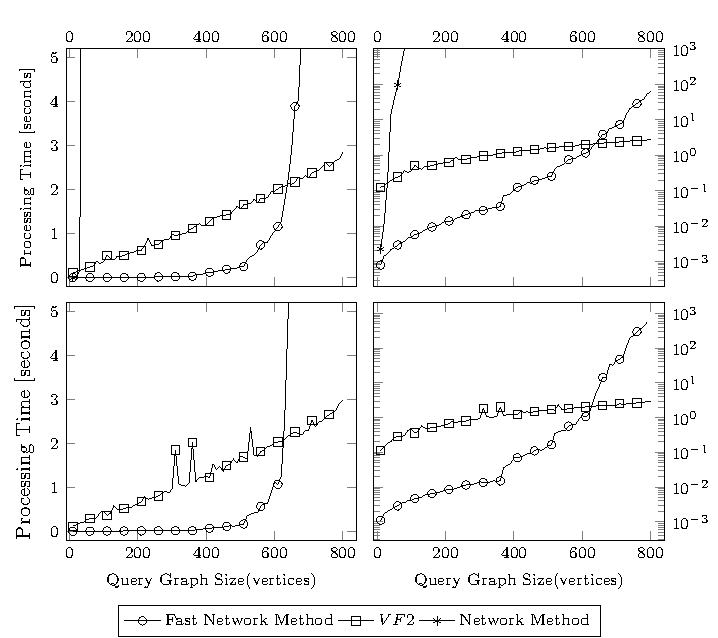
\includegraphics[width=1.0\textwidth]{syndataplot.pdf}
\caption{\textbf{Results of the Experiments on the Synthetic Graph Data Set} 

\textbf{ Top left:}Linear-linear plot of induced subgraph query processing time against query graph vertex count. The query graph size ranges from 10 vertices to 800 vertices. The \textit{Fast Network Method} and the \textit{Network Method} show the fastest processing time for induced subgraph queries of up to 600 vertices. For larger query graphs, the \textit{VF2} method is faster. The \textit{Network Method} takes more than 5sec for any induced subgraph query graph greater than 10 vertices. The \textit{VF2} method shows an almost linear time dependency of query graph vertex count, an advantage for induced subgraph queries larger than 600 vertices. 

\textbf{Top Right:} Linear-log plot of the induce subgraph graph query processing time with query graph size. We observe that for induced subgraph query size less than 400 Vertices, there is an order of magnitude or better advantage to the \textit{Fast Network Method}. Beyond query graphs of about 600 vertices the \textit{VF2} method is clearly superior. We observe that the \textit{Network Method} is slowest, taking about 15min for an induced subgraph query of just 80 vertices.

\textbf{ Bottom left:}Linear-linear plot of  query processing time for increasing size of graph query.The smallest query graph contains 10 vertices while the largest query graph contains 800 vertices. The \textit{Fast Network Method} processes query graphs faster than \textit{VF2} for subgraphs not larger than 600 vertices. Here too, \textit{VF2} method shows an almost linear processing time  dependency with query graph size.  

\textbf{Bottom Right:} Linear-log plot of the induce subgraph graph query processing time with query graph size. For subgraph query size less than about 400 Vertices, there is an order of magnitude or better advantage to the \textit{Fast Network Method}. For synthetic graphs of less that 50 vertices, the advantage is about two orders of magnitude. Beyond query graphs of about 600 vertices the \textit{VF2} method is superior.
}
\label{fig:fig91}
\end{figure}
%

%Fig.\ref{fig:fig5} shows the processing time for induced subgraph isomorphism query.
%Fig.\ref{fig:fig5} indicates that proposed algorithm is faster than Messmer et al.'s algorithm.
%The processing time of proposed algorithm is stable against the variation of the size of query graphs.
%On the contrary, the processing time of Messmer et al.'s algorithms is skyrockets when the size of query graphs becomes large.

% LocalWords:  kna


\section{Conclusions}
In this article, we have studied the problem of scalable enumeration of all subgraph isomorphisms in a graph database. We took the graph decomposition process of the \textit{Network Algorithm} first proposed by  Messmer and Bunke \cite{messmer_bunke2000} and extended it from processing only induced subgraph isomorphism to include subgraph isomorphism. The extended Algorithm  likely suits more research oriented as well as real world  problems.
We proposed improvements on \textit{Network Algorithm} enable it to process larger query or a larger graph database while maintaining good performance.
We did this mainly by restraining the rapid increase in running time due to the creation of disconnected graphs in the DAG during query processing.

For small graphs our method shows performance that is indistinguishable from that is Messmer's \textit{Network Algorithm}. We have shown that for large
query graph and for large database our method is an order of magnitude faster than the \textit{Network Algorithm} or VF2. This is in spite of the fact that, unlike
VF2 algorithm, our algorithm processes enumeration of all isomorphic subgraphs, while VF2 will stop as soon as an isomorphic subgraph is detected in the database.





%\End{document}  % This is where a 'short' article might terminate

% Acknowledgments
%\begin{acks}
%The authors would like to thank Dr. Maura Turolla of Telecom
%Italia for providing specifications about the application scenario.
%\end{acks

%% Bibliography
\bibliographystyle{acmsmall}
\bibliography{master}
%

%\balancecolumns % GM July 2000
% That's all folks!
\end{document}

% LocalWords:  Katayama LocalWords truein
 
